\documentclass[article,nojss]{jss}
%% need no \usepackage{Sweave}
%\documentclass[article]{jss}
\usepackage{thumbpdf,lmodern} 
\graphicspath{{Figures/}}

\usepackage{amsmath}

\author{
	Felix Pretis\\University of Victoria \\ \& University of Oxford \And
	J. James Reade\\ University of Reading \And
	Genaro Sucarrat\\BI Norwegian Business School
}

\title{An introduction to the \textit{gets} package\thanks{Date: 7 September 2020. This paper is almost an exact reproduction of our paper on the package published in Journal of Statistical Software: \url{https://doi.org/10.18637/jss.v086.i03}}}

%OLD/ORIGINAL:
%\title{Automated General-to-Specific (GETS) Regression Modeling and Indicator Saturation for Outliers and Structural Breaks\thanks{This paper is almost an exact reproduction of our paper on the package published in Journal of Statistical Software: \url{https://doi.org/10.18637/jss.v086.i03}}}

\Plainauthor{Felix Pretis, J. James Reade, Genaro Sucarrat} 

\Shorttitle{\pkg{gets}: General-to-Specific Modeling and Indicator Saturation}

\Abstract{ This paper provides an overview of the \proglang{R} package
  \pkg{gets}, which contains facilities for automated
  general-to-specific (GETS) modeling of the mean and variance of a
  regression, and indicator saturation (IS) methods for the detection
  and modeling of outliers and structural breaks. The mean can be
  specified as an autoregressive model with covariates (an ``AR-X''
  model), and the variance can be specified as an autoregressive
  log-variance model with covariates (a ``log-ARCH-X'' model). The
  covariates in the two specifications need not be the same, and the
  classical linear regression model is obtained as a special case when
  there is no dynamics, and when there are no covariates in the
  variance equation. The four main functions of the package are
  \code{arx}, \code{getsm}, \code{getsv} and \code{isat}. The first
  function estimates an AR-X model with log-ARCH-X errors. The second
  function undertakes GETS modeling of the mean specification of an
  `\code{arx}' object. The third function undertakes GETS modeling of
  the log-variance specification of an `\code{arx}' object. The fourth
  function undertakes GETS modeling of an indicator-saturated mean
  specification allowing for the detection of outliers and structural
  breaks. The usage of two convenience functions for export of results
  to \proglang{EViews} and \proglang{STATA} are illustrated, and \LaTeX{} code of
  the estimation output can readily be generated.  }
      
\Keywords{general-to-specific, model selection, variable selection, regression of the mean, regression of the log-variance, time series, AR-X, log-ARCH-X, indicator saturation, \proglang{R}}

\Plainkeywords{general-to-specific, model selection, variable selection, regression of the mean, regression of the log-variance, time series, AR-X, log-ARCH-X, indicator saturation, R}

\Address{
	Felix Pretis\\
	University of Victoria, Department of Economics \\
	\& INET at the Oxford Martin School, University of Oxford\\
	E-mail: \email{fpretis@uvic.ca}\\
	URL: \url{http://www.felixpretis.org/}  
	
	J. James Reade\\
	Programme for Economic Modelling at the Oxford Martin School \\
	\& Department of Economics
	University of Reading\\
	E-mail: \email{j.j.reade@reading.ac.uk}\\
	URL: \url{https://sites.google.com/site/jjamesreade/}
	
	Genaro Sucarrat\\
	Department of Economics\\
	BI Norwegian Business School\\
	0484 Oslo, Norway\\
	E-mail: \email{genaro.sucarrat@bi.no}\\
	URL: \url{http://www.sucarrat.net/}
}
\begin{document}

%\SweaveOpts{engine=R,eps=FALSE}
%\VignetteIndexEntry{An introduction to the gets package}
%\VignetteDepends{gets}
%\VignetteKeywords{general-to-specific, model selection, variable selection, regression of the mean, regression of the log-variance, time series, AR-X, log-ARCH-X, indicator saturation}
%\VignettePackage{gets}

\section{Introduction}

General-to-specific (GETS) modeling combines well-known ingredients:
backwards elimination, single and multiple hypothesis testing,
goodness-of-fit measures and diagnostics tests. The way these are
combined by GETS modeling enables rival theories and models to be
tested against each other, ultimately resulting in a parsimonious,
statistically valid model that explains the characteristics of the
data being investigated. The methodology thus provides a systematic
and coherent approach to model development and maintenance, cumulative
research and scientific progress. This paper provides an overview of
the \proglang{R} \citep{RCoreTeam2016} package \pkg{gets}
\citep{gets}, which contains facilities for automated
general-to-specific (GETS) modeling of the mean and variance of
cross-sectional and time-series regressions, and indicator saturation
(IS) methods for the detection and modeling of outliers and structural
breaks in the mean.

The origins of GETS modeling can be traced back to Denis Sargan and
the London School of Economics (LSE) during the 1960s, see
\cite{Hendry03} and \cite{Mizon95}. However, it was not until the
1980s and 1990s that the methodology gained widespread acceptance and
usage in economics, with David F.~Hendry in particular being a main
proponent, see the two-volume article collection by
\cite{CamposEricssonHendry2005} for a comprehensive overview of the
GETS methodology. An important software-contribution to GETS modeling
was made in 1999, when \cite{Hooveretal99} re-visited the data-mining
experiment of \cite{Lovell83}. \cite{Hooveretal99} showed that
automated multi-path GETS modeling substantially improved upon the
then (in economics) popular model selection strategies. In the study
of \cite{Hooveretal99}, purpose-specific but limited \proglang{MATLAB}
\citep{MATLABR2017b} code was used in the simulations.\footnote{The
  code is limited in that it allows for a maximum of 10 paths to be
  searched, and because there is no user manual nor help-system
  available. The data and \proglang{MATLAB} code is available from
  \url{http://www.feweb.vu.nl/econometriclinks/journal/volume2/HooverKD_PerezSJ/data_and_code/}.}
Subsequently, further improvements were achieved in the commercial
software packages \pkg{PcGets} \citep{Hendryetal01} and in its
successor \pkg{Autometrics} \citep{DoornikHendry2007}. In particular,
indicator-saturation methods for the detection of outliers and
structural breaks proposed by \cite{HendryJohansenSantos2007} were
added to \pkg{Autometrics} in 2008, see \cite{Doornik2009}. Another
milestone was reached in 2011, when the \proglang{R} package
\pkg{AutoSEARCH} \citep{AutoSEARCH} was published on the Comprehensive
\proglang{R} Archive Network (CRAN). The package, whose code was
developed based on \cite{SucarratEscribano2012}, offered automated
GETS modeling of conditional variance specifications within the
log-ARCH-X class of models. The \proglang{R} package \pkg{gets},
available from CRAN since October 2014, is the successor of
\pkg{AutoSEARCH}. The \pkg{gets} package, at the time of writing, is
the only statistical software that offers GETS modeling of the
conditional variance of a regression, in addition to GETS modeling of
the mean of a regression, and indicator saturation (IS) methods for
the detection of breaks of outliers structural breaks in the mean of a
regression using impulses (IIS), step (SIS; see
\citealt{castle2015detecting}) as well as trend indicators (TIS).

This paper provides an overview of the \pkg{gets} package. The main
model class under consideration is the autoregressive (AR) model with
exponential autoregressive conditional heteroscedastic (ARCH)
variance, possibly with additional covariates in the mean or variance
equations, or in both.  In short, the AR-X model with a log-ARCH-X
error term, where the ``X'' refers to the covariates (the covariates
need not be the same in the mean and variance specifications). It
should be underlined, however, that \pkg{gets} is not limited to
time-series models (see Section~\ref{subsec:development:principles}):
Static models (e.g., cross-sectional or panel) can be estimated by specifying
the regression without dynamics. The next section,
Section~\ref{sec:an:overview}, provides an overview of GETS modeling
and its alternatives, and outlines the principles that guides the
development of
\pkg{gets}. Section~\ref{sec:setting:time:series:attributes} contains
a note on the advantage of providing the data with time-series
attributes -- if the data are indeed time-series, since this is useful
for the estimation of dynamic models, output and
graphing. Section~\ref{sec:ar-x:model:with:log-arch-x:errors} contains
an overview of the AR-X model with log-ARCH-X errors, explains how it
can be simulated, and illustrates how it can be estimated with the
\code{arx} function. Section~\ref{sec:gets:model:selection}
illustrates how GETS modeling can be undertaken with the \code{getsm}
and \code{getsv} functions. The first undertakes GETS modeling of the
mean specification, whereas the second undertakes GETS modeling of the
log-variance specification. Section~\ref{sec:indicator:saturation}
introduces the \code{isat} function for indicator saturation
methods. Section~\ref{sec:eviews:and:stata:export} illustrates how two
convenience functions, \code{eviews} and \code{stata}, facilitate GETS
modeling by users of \proglang{EViews} \citep{EViews2016v9.5} or
\proglang{STATA} \citep{STATA2017}, i.e., the two most popular
commercial software packages in econometrics. The section also briefly
alludes to how estimation output can readily be converted into
\LaTeX{} code. Finally, Section~\ref{sec:conclusions} concludes.

\section{An overview, alternatives and development principles}
\label{sec:an:overview}

\subsection{GETS modeling}
\label{subsec:gets:modeling}

It is convenient to provide an overview of GETS modeling in terms of the linear regression model
%
\begin{equation}\label{eq:linear:regression:model}
y_t = \beta_1 x_{1t} + \cdots + \beta_k x_{kt} + u_t, \qquad t=1,2,\ldots, n,
\end{equation}
%
where $y_t$ is the dependent variable, the $\beta$'s are slope
coefficients, the $x$'s are the regressors and $u_t$ is a zero mean
error term. GETS modeling assumes there exists at least one ``local''
data generating process (LDGP) nested in
(\ref{eq:linear:regression:model}). By philosophical assumption $the$
DGP is not contained in the simple model above, see
\cite{Sucarrat2010} and \citet[][Sections
6.2--6.3]{HendryDoornik2014}. The qualifier ``local'' thus means it is
assumed that there exists a specification within
(\ref{eq:linear:regression:model}) that is a statistically valid
representation of $the$ DGP. Henceforth, for notational and
theoretical convenience, we will assume there exists only a single
LDGP, but this is not a necessary condition.

A variable $x_{jt}$, $j\in \{1,\ldots,k\}$, is said to be relevant if $\beta_j \neq 0$ and irrelevant if $\beta_j = 0$. Let $k_{\text{rel}} \geq 0$ and $k_{\text{irr}} \geq 0$ denote the number of relevant and irrelevant variables, respectively, such that $k_{\text{rel}} + k_{\text{irr}} = k$. Of course, both $k_{\text{rel}}$ and $k_{\text{irr}}$ are unknown to the investigator. GETS modeling aims at finding a specification that contains as many relevant variables as possible, and a proportion of irrelevant variables that corresponds to the significance level $\alpha$ chosen by the investigator. Put differently, if $\widehat{k}_{\text{rel}}$ and $\widehat{k}_{\text{irr}}$ are the retained number of relevant and irrelevant variables, respectively, then GETS modeling aims at satisfying 
%
\begin{equation}
\E(\widehat{k}_{\text{rel}}/k_{\text{rel}}) \rightarrow 1 \quad \textnormal{and} \quad \E(\widehat{k}_{\text{irr}}/k_{\text{irr}}) \rightarrow \alpha \quad \textnormal{as} \quad n\rightarrow\infty,
\end{equation}
%
when $k_{\text{rel}},k_{\text{irr}}>0$.  If either $k_{\text{rel}}=0$
or $k_{\text{irr}}=0$, then the criteria are modified in the obvious
ways: If $k_{\text{rel}}=0$, then $\E(\widehat{k}_{\text{rel}}) = 0$,
and if $k_{\text{irr}}=0$, then $\E(\widehat{k}_{\text{irr}}) =
0$. The proportion of spuriously retained variables, i.e.,
$\widehat{k}_{\text{irr}}/k_{\text{irr}}$, is also referred to as
\textit{gauge} in the GETS literature, with distributional results on
the gauge for a specific case (the variables being impulses as in IIS)
provided in \cite{johansen2016asymptotic}. The relevance proportion,
i.e., $\widehat{k}_{\text{irr}}/k_{\text{irr}}$, is also referred to
as \textit{potency} in the GETS
literature. Table~\ref{table:comparison:of:gets:algorithms} contains a
comparison of the variable selection properties of GETS software
packages for some well-known experiments. As the results show,
\pkg{gets} performs as expected in the experiments, since the
irrelevance proportion corresponds well to the nominal regressor
significance level $\alpha$, and since the relevance proportion is
1. Additional simulations, and comparisons against alternative
algorithms, are contained in
Section~\ref{subsec:comparison:of:gets:with:alternatives}.

\begin{table}[t!]
  \centering
  \begin{tabular}{lcclrccc}
    \hline
		Experiment & $k_{\text{rel}}$ & $k_{\text{irr}}$ & Algorithm & $n$ & $m(\widehat{k}_{\text{rel}}/k_{\text{rel}})$ & $m(\widehat{k}_{\text{irr}}/k_{\text{irr}})$ & $\widehat{p}(\text{DGP})$ \\
		\hline
		HP1 & 0 & 40 & \pkg{gets} & 139 &  & 0.053 & 0.269 \\
		& & & \pkg{AutoSEARCH} & &  & 0.049 & 0.239 \\
		&  &  & HP1999 &  &  & 0.045 & 0.292 \\
		&  &  & \pkg{PcGets} &  &  & $\approx 0.04$ & $\approx 0.45$ \\[2mm]
		%
		HP2' & 1 & 39 & \pkg{gets} & 139 & 1.000 & 0.056 & 0.254 \\
		& & & \pkg{AutoSEARCH} & & 1.000 & 0.050 & 0.252 \\
		&  &  & HP1999 &  & 1.000 & 0.107 & 0.000 \\
		&  &  & \pkg{PcGets} &  & $\approx 0.97$ & $\approx 0.05$ & $\approx 0.32$ \\
		&  &  & \pkg{Autometrics} &  & 1.000 & 0.063 & 0.119 \\[2mm]
		%
		HP7' & 3 & 37 & \pkg{gets} & 138 & 0.999 & 0.055 & 0.232 \\
		& & & \pkg{AutoSEARCH} & & 1.000 & 0.051 & 0.232 \\
		&  &  & HP1999 &  & 0.967 & 0.082 & 0.040 \\
		&  &  & \pkg{PcGets} &  & $\approx 1.00$ & $\approx 0.04$ & $\approx 0.37$ \\
		&  &  & \pkg{Autometrics} &  & 0.999 & 0.066 & 0.111 \\
		\hline
	\end{tabular}
	\caption{Variable selection properties of GETS algorithms. The
          table is essentially Table 2 in
          \citet[][p.~724]{SucarratEscribano2012} augmented by the
          properties of \pkg{gets}, see Appendix~\ref{appendix} for more details
          on the simulations. The variable selection is undertaken
          with a nominal regressor significance level of
          5\%. $m(\widehat{k}_{\text{rel}}/k_{\text{rel}})$, average
          proportion of relevant variables $\widehat{k}_{\text{rel}}$
          retained relative to the actual number of relevant variables
          $k_{\text{rel}}$.
          $m(\widehat{k}_{\text{irr}}/k_{\text{irr}})$, average
          proportion of irrelevant variables
          $\widehat{k}_{\text{irr}}$ retained relative to the actual
          number of irrelevant variables $k_{\text{irr}}$ in the
          GUM. $\widehat{p}(\text{DGP})$, proportion of times the
          exact DGP is found. The properties of the HP1999 algorithm
          are from \citet[][Table 4 on p.~179]{Hooveretal99}. The
          properties of the \pkg{PcGets} algorithm are from
          \citet[][Figure 1 on p.~C39]{HendryKrolzig2005}, and the
          properties of the \pkg{Autometrics} algorithm are from
          \citet[][Section
          6]{Doornik2009}. \label{table:comparison:of:gets:algorithms}
        }
\end{table}

GETS modeling combines well-known ingredients from the model-selection literature: backwards elimination, tests on the $\beta_j$'s (both single and multiple hypothesis tests), diagnostics tests, and fit-measures (e.g., information criteria). Specifically, GETS modeling may be described as proceeding in three steps:

\begin{enumerate}
	\item Formulate a general unrestricted model (GUM) that passes a set of chosen diagnostic tests.\footnote{Currently, the standard diagnostic tests available in \pkg{gets} are tests for serial correlation and ARCH in the standardized residuals, and a test for non-normality. In addition, the user may add her or his own test or set of tests via the \code{user.diagnostics} argument.} Each non-significant regressor in the GUM constitutes the starting point of a backwards elimination path, and a regressor is non-significant if the $p$~value of a two-sided $t$-test is lower than the chosen significance level $\alpha$.
	
	\item Undertake backwards elimination along multiple paths by removing, one-by-one, non-significant regressors as determined by the chosen significance level $\alpha$. Each removal is checked for validity against the chosen set of diagnostic tests, and for parsimonious encompassing (i.e., a multiple hypothesis test) against the GUM.
	
	\item Select, among the terminal models, the specification with the best fit according to a fit-criterion, e.g., the \cite{Schwarz1978} information criterion. 
\end{enumerate}

For $k$ candidate variables, there are $2^k$ possible models. As $k$ becomes large the number of models becomes computationally infeasible, thus, a structured search is required. GETS provides such a structured search by starting with a general model (the GUM), and subsequently removing variables along search paths while checking the diagnostics at each removal.

\subsection[A comparison of GETS and gets with alternatives]{A comparison of GETS and \pkg{gets} with alternatives}
\label{subsec:comparison:of:gets:with:alternatives}

When comparing the \proglang{R} package \pkg{gets} to alternatives, it is important to differentiate the methodological approach of GETS modeling relative to other modeling approaches, from different software implementations within the GETS methodology. Here, we denote the broader field of GETS modeling by GETS, and the \proglang{R} package by \pkg{gets}. First we briefly review and compare alternative approaches to GETS modeling, then we discuss alternative implementations of GETS.

\subsubsection{GETS compared to alternative methods -- a feature-based comparison}
\label{sec:GETSalt}

Numerous model and variable selection methods have been proposed, and
an even larger number of implementations are available. Focusing on
variable selection, Table~\ref{table:comparison:of:softwares} contains
a feature-based comparison of \pkg{gets} against some common
alternatives in \proglang{R}. The \code{ar} function in \pkg{stats}
\citep{RCoreTeam2016} searches for the best AR($P$) model using the
AIC. The \code{step} function, also in \pkg{stats}, offers both
forward and backward step-wise search. The packages \pkg{lars}
\citep{HastieEfron2013} and \pkg{glmnet}
\citep{friedman2010regularization}, provide shrinkage-based search
methods for variable selection.

As is clear from the table, GETS may be viewed as being more general than many of its competitors. This comes at a cost: computational speed. Relying on multiple path searches implies that the required computational time increases non-linearly with the number of potential candidate regressors selected over. This is a particular concern when using indicator saturation (Section~\ref{sec:indicator:saturation}), where the number of candidate variables scales linearly with the number of observations and subsequently implies a non-linear increase in required computational time. For example, selection over $k$ (irrelevant) candidate regressors in \pkg{gets} (in a sample of $n=200$ observations) on a 1.8GHz processor requires approximately 0.8 seconds (s) for $k=10$, 2.9s for $k=20$, 15s for $k=40$, and 114s for $k=80$. By contrast, the identical experiment with $k=80$ requires 0.16s using the Lasso in \pkg{glmnet}, 0.41s in \pkg{lars}, and 0.3s using \code{step} (backward).

\begin{table}[t!]
	\centering
	\begin{tabular}{lcccccc}
		\hline
		& \code{ar} & \code{step} (forward) & \code{step} (backward) & \pkg{lars} & \pkg{glmnet} & \pkg{gets} \\
		\hline
		AR-terms & Yes & Yes & Yes & Yes & Yes & Yes \\[1mm] 
		Covariates (``X'') & & Yes & Yes & Yes& Yes & Yes \\[1mm] 
		More variables & & & & & & \\ 
		than observations & & Yes & & Yes & Yes & Yes \\[1mm] 
		Variance-modeling & & & & & & Yes \\[1mm] 
		Regressor tests & & & & & & \\
		during search & & & & & & Yes \\[1mm] 
		Diagnostics tests & & & & & & \\
		during search & & & & & & Yes \\[1mm] 		
		Computational & & & & & & \\ 		
		cost (relative) & Low & Low & Low & Low & Low & High \\[1mm] 		
		\hline
	\end{tabular}\\
	%	\raggedright
	\caption{A variable-selection focused feature-based comparison of \pkg{gets}  against the \code{ar} and \code{step} functions in the \proglang{R} package \pkg{stats} \citep{RCoreTeam2016}, and against the \proglang{R} packages \pkg{lars} \citep{HastieEfron2013} and \pkg{glmnet} \citep{friedman2010regularization}. \label{table:comparison:of:softwares} }
\end{table}

\subsubsection{GETS compared to alternative methods -- a performance-based comparison}

\citet[Section 17]{HendryDoornik2014} together with
\cite{castle2011evaluating} provide a broad overview of the
performance of GETS relative to alternative model selection strategies
of the mean of a regression, including step-wise regression,
information criteria and penalized shrinkage-based selection using the
Lasso
\citep[see][]{tibshirani1996regression}. \cite{castle2015detecting}
compare GETS in the context of step-shifts against the Lasso using
LARS \citep{efron2004least}, and \cite{pretis_volc16} compare GETS
against the Lasso for designed break functions (see
Section~\ref{sec:isat_comp} for a more detailed discussion of
\pkg{gets} in the context of break detection). In both instances
shrinkage-based selection is implemented using the \proglang{R}
packages \pkg{lars} \citep{HastieEfron2013} and \pkg{glmnet}
\citep{friedman2010regularization}.  The emerging consensus from these
simulation comparisons is that the false-positive rate, or irrelevance
proportion or gauge, is erratic and difficult to control in step-wise
as well as shrinkage-based selection procedures. When selecting on
information criteria only, the implicit significance level of
selection results in a high gauge when the number of candidate
variables increases relative to the sample size. In contrast, the
gauge tends to be well-calibrated around the nominal size of selection
$\alpha$ in GETS.  While the retention of relevant variables often is
high in shrinkage-based approaches (and erratic in step-wise
regression), this result comes at the cost of a high gauge and the
performance becomes less reliable in the presence of correlation
between the candidate variables.

To provide additional comparisons of performance to alternative
methods for detecting relevant and discarding irrelevant variables,
here we compare \pkg{gets} to: shrinkage-based selection, 1-cut
selection (where all variables with $p$~values $\leq \alpha$ in the GUM
are retained in a single decision), and conducting selection inference
starting at the DGP itself. The results are provided in
Figure~\ref{fig_lass} (and Tables~\ref{tab_lassuncorr},
\ref{tab_lassposcorr}, and \ref{tab_lassnegcorr} in Appendix~\ref{sec:simulation-tables}). The
simulations cover three correlation structures of regressors: First,
in-expectation uncorrelated regressors, second, positively correlated
regressors ($\rho=0.5$), and third, alternating negatively correlated
regressors (where $\rho(x_i, x_{i+1}) = 0.5$,
$\rho(x_i, x_{i+2})=-0.5$). We consider a total of $k=20$ regressors
in a sample of $n=500$ observations for $1000$ replications. The
number of relevant regressors is increased from $k_{\text{rel}}=0$ to
$k_{\text{rel}}=10$ with coefficients set to correspond to an expected
$t$-statistic of $\approx 3$. The performance of \pkg{gets} using the
\code{getsm} function is compared to the cross-validated Lasso in
\pkg{glmnet} and the Lasso with fixed penalty parameter such that the
false-detection rate approximately matches \code{getsm} under the null
(when $k_{\text{rel}}=0$). The significance level of 1-cut selection
is chosen to match $\alpha=1\%$ in \code{getsm} selection.

\begin{figure}[t!]
  \centering
  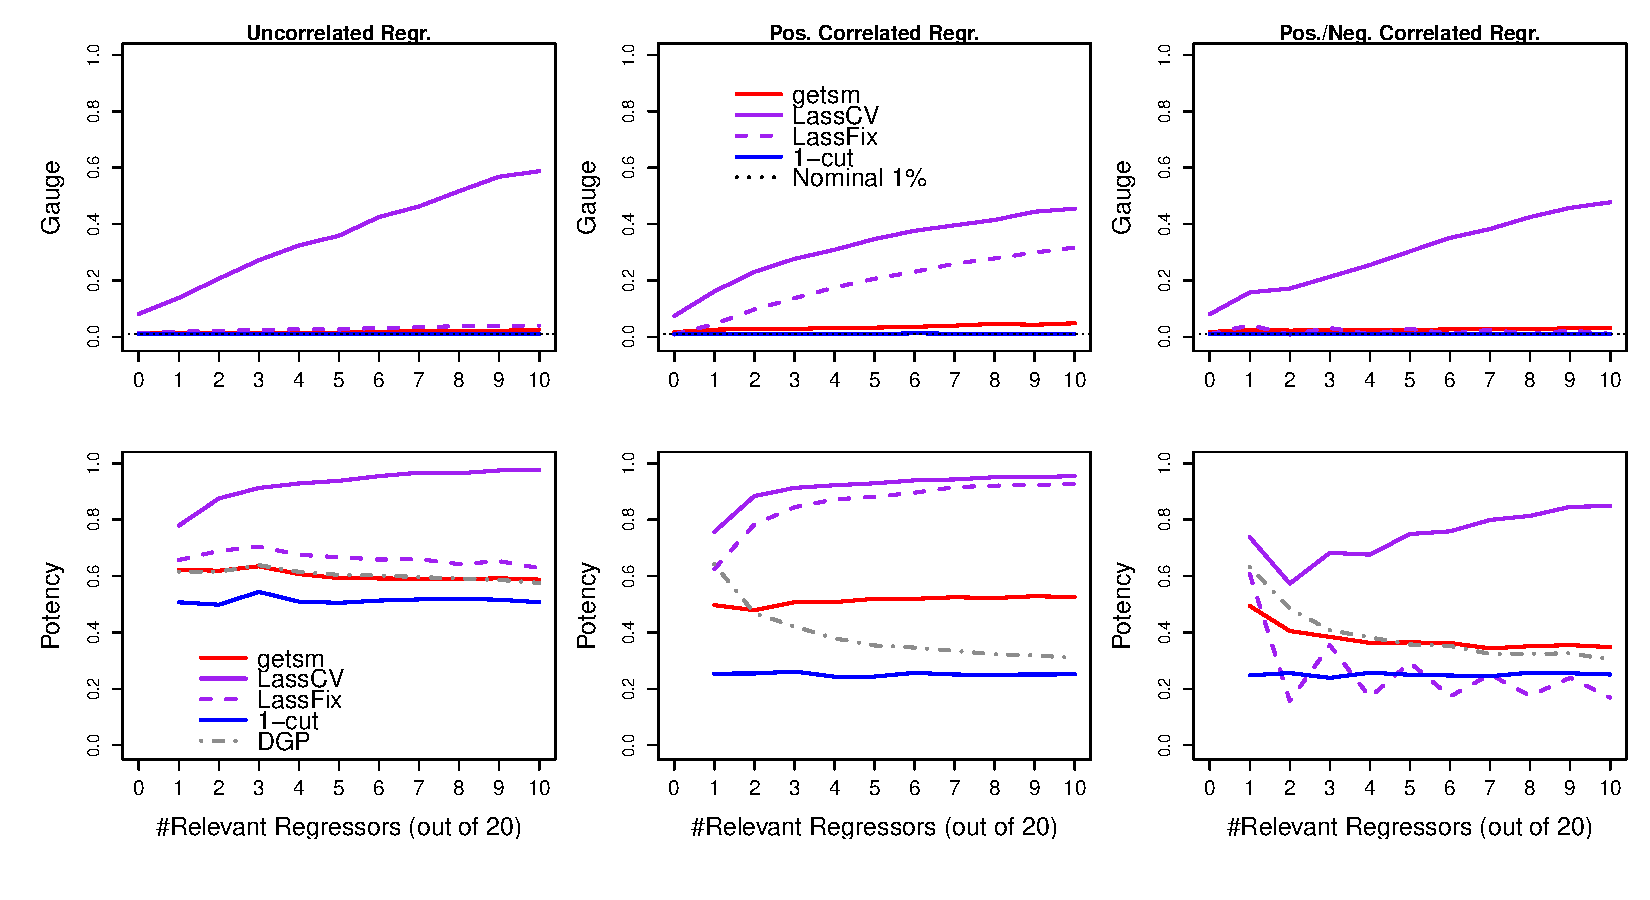
\includegraphics[width=\textwidth, trim = 0 0 0 0, clip]{fig_getsm_performance_v2.pdf}
  \caption{Performance of \code{getsm} selection algorithm compared
    against alternatives: cross-validated Lasso (LassCV), Lasso with
    fixed penalty (LassFix), 1-cut selection, and significance in the
    DGP itself (DGP). The top row shows the false retention rate (gauge),
    the bottom row shows the correct retention of relevant variables
    (potency). Columns show uncorrelated, positively correlated, and
    alternating positively and negatively correlated
    regressors. Nominal selection in \code{getsm} taken place at 1\%
    significance level. \label{fig_lass} }
\end{figure}

The simulation results presented here match the evidence from previous studies: GETS selection yields a false-detection rate close to the nominal size of selection regardless of the correlation structure of regressors considered. While exhibiting high potency, the false detection rate of Lasso is difficult to control when the correlation structure varies and the number of relevant variables is unknown. GETS dominates 1-cut selection when regressors are correlated, and closely matches 1-cut in absence of correlation.

To the best of our knowledge, the only currently publicly available software that provides automated model selection of the variance is \pkg{gets}. The reason for this is that \pkg{gets} sidesteps the numerical estimation difficulties usually associated with models of the variance thanks to its OLS estimation procedure, see the discussion in \cite{SucarratEscribano2012}.

\subsubsection{Alternatives within the field of GETS}
\label{sec:getsalt}

There have been different software implementations of GETS modeling --
Table~\ref{table:feature-comparison:of:gets:softwares} summarizes the
similarities and differences between these. The main (currently
available) alternative to the package \pkg{gets} for GETS modeling of
the mean in regression models is \pkg{Autometrics} \citep{Doornik2009}
written in \proglang{Ox} \citep{Doornik2006} within the software
package \pkg{PcGive} \citep{DoornikHendry2007a}. \pkg{Autometrics} and
\pkg{gets} share common features in GETS modeling of the mean in
regression models, and in the general implementation of impulse- and
step-indicator saturation. There are, however, notable differences
between the two implementations: The main advantages of \pkg{gets} lie
in being the only GETS implementation of variance models, the
implementation of new and unique features in indicator saturation
methods including trend-indicator saturation (TIS), consistency and
efficiency corrections of the variance estimates, and testing of the
time-varying mean (see Section~\ref{sec:isat_comp} for an in-depth
discussion of the differences in indicator saturation between
\pkg{Autometrics} and \pkg{gets}), as well as new features in model
selection (e.g., the availability of a direct function to correct for
model-selection bias). In turn, selection over systems of equations
can be conducted automatically in \pkg{Autometrics} while having to be
done by one-equation at a time in \pkg{gets}.

\begin{table}[t!]
	\centering
	\begin{tabular}{lccccc}
		\hline
		& & HP1999 & \pkg{PcGets} & \pkg{Autometrics} & \pkg{gets} \\
		\hline
		More than 10 paths & &  & Yes & Yes & Yes \\[1mm] 
		GETS of mean & & Yes & Yes & Yes & Yes \\[1mm]
		GETS of variance & &  &  &  & Yes \\[1mm]
		Impulse and step IS & &  &  & Yes & Yes \\[1mm]
		Trend IS  & &  &  &  & Yes \\[1mm]
		IS variance correction		& &  &  &  & Yes \\[1mm]
		User-defined diagnostics & &  &  &  & Yes \\[1mm]
		GETS of logit models 		 & &  &  & Yes &  \\[1mm]
		GETS of systems & &  &  & Yes &  \\[1mm]	
		Menu-based GUI  & &  & Yes & Yes &  \\[1mm]		
		Free and open source & & Yes &  &  & Yes \\[1mm]
		\hline
	\end{tabular}\\
	\caption{A feature-based comparison of GETS software packages;
          the \proglang{MATLAB} code of \cite{Hooveretal99} (HP1999),
          \pkg{PcGets} version 0.9, \pkg{Autometrics} version 7 and
          \pkg{gets} version
          0.12. \label{table:feature-comparison:of:gets:softwares} }
\end{table}

\subsection[Development principles of the package gets]{Development principles of the package \pkg{gets}}
\label{subsec:development:principles}

The original motivation behind the precursor of \pkg{gets} (i.e.,
\pkg{AutoSEARCH}) was to make GETS modeling methods of the variance
(and mean) of a regression freely and publicly available, while being
open-source and implementing recent developments in GETS. This
principle will continue to guide the development of
\pkg{gets}. Indicator saturation methods were added to \pkg{gets} in
version 0.2, and we plan to expand \pkg{gets} further to include model
classes for which there currently is no GETS software, e.g., spatial
models, panel-data, etc. Naturally, we encourage others keen to develop
and publish GETS modeling methods for a wider range of alternatives, 
either within the \pkg{gets} package or as a separate package. Another important
development principle is that we would like to enable more
user-specified control. User-specified diagnostics, for example, were
added in version 0.10, and we also plan to enable user-specified
estimation and inference procedures (this is already available in
\code{arx}, but not in \code{getsm}, \code{getsv} and
\code{isat}). Finally, we also aim at making the package
computationally faster and more user-friendly.

\section{Setting time-series attributes}
\label{sec:setting:time:series:attributes}

The \pkg{gets} package is not limited to time series models and does
not require that time-series characteristics are set beforehand (for
example if the data at hand are not time series). However, if time
series characteristics are not set, and if the data are in fact time
series, then graphs and other outputs (e.g., fitted values, residuals,
etc.) are not optimal. The \pkg{gets} package is optimized to work
with Z's ordered observations (ZOO) package \pkg{zoo}, see
\cite{ZeileisGrothendieck2005}. In fact, the fitted values, residuals,
recursive estimates and so on returned by \pkg{gets} functions, are
all objects of class `\code{zoo}'. The \pkg{zoo} package provides a very
general and versatile infrastructure for observations that are ordered
according to an arbitrary index, e.g., time-series, and \pkg{zoo} is
adapted to interact well with the less versatile time-series class of
the \pkg{base} distribution, `\code{ts}': To convert `\code{ts}' objects
to `\code{zoo}' objects, simply use \code{as.zooreg} (preferred) or
\code{as.zoo}. See the help system and webpage of the \pkg{zoo}
package for several short intros and vignettes:
\url{https://CRAN.R-project.org/package=zoo}.

\section{The AR-X model with log-ARCH-X errors}
\label{sec:ar-x:model:with:log-arch-x:errors}

The specifications considered by \pkg{gets} are all contained in the AR-X model with log-ARCH-X errors. This model is made up of two equations, one for the mean and one for the log-variance:
%
\begin{eqnarray}
	y_t &=& \phi_0 + \sum_{r=1}^R \phi_r y_{t-r} + \sum_{s=1}^S\eta_s x_{s,t}^m + \epsilon_t, \qquad \epsilon_t = \sigma_tz_t, \quad z_t \sim \text{iid}(0,1), \label{eq:ar-x} \\
	%
	\nonumber \ln\sigma_t^2 &=& \alpha_0 + \sum_{p=1}^P \alpha_p \ln\epsilon_{t-p}^2 + \sum_{q\in Q} \beta_q \ln \text{EqWMA}_{q,t-1} \\
	%
	&& + \sum_{a=1}^A \lambda_a(\ln\epsilon_{t-a}^2)I_{\{\epsilon_{t-a} < 0\}} + \sum_{d=1}^D\delta_d x_{d,t}^v. \label{eq:log-variance}
\end{eqnarray}
%
The conditional mean equation (\ref{eq:ar-x}) is an autoregressive
(AR) specification of order $R$ with $S$ covariates
$x_{1,t}^m, \ldots, x_{S,t}^m$ (``X''), AR-X for short. The covariates
may contain lags of conditioning variables. The error term
$\epsilon_t$ is a product of the time-varying conditional standard
deviation $\sigma_t > 0$ and the real-valued innovation $z_t$, where
$z_t$ is iid with zero mean and unit variance conditional on the
past. The conditional log-variance equation (\ref{eq:log-variance}) is
given by a logarithmic autoregressive conditional heteroscedasticity
(log-ARCH) specification of order $P$ with volatility proxies defined
as $\text{EqWMA}_{q,t-1} = (\epsilon_{t-1}^2 + \cdots + \epsilon_{t-q}^2)/q$,
$A$ logarithmic asymmetry terms (i.e., ``leverage'') analogous to those
of \cite{GlostenJagannathanRunkle1993} -- so $I_{\epsilon_{t-a} < 0}$
is an indicator function equal to 1 if $\epsilon_{t-a} < 0$ and 0
otherwise, and $D$ covariates $x_{1,t}^v, \ldots, x_{D,t}^v$,
log-ARCH-X for short. The covariates may contain lags of conditioning
variables, and the covariates in the mean need not be the same as
those of the log-variance specification. Hence the superscripts $m$
and $v$, respectively. The log-proxies $\ln \text{EqWMA}_{q,t-1}$, where
EqWMA is short for equally weighted moving average, are intended to
proxy lagged log-GARCH terms, e.g., $\ln\sigma_{t-1}^2$. However, it
should be noted that the log-proxies can also be given additional
interpretation of interest. For example, if $y_t=\epsilon_t$ is a
daily financial return, and if the returns are recorded over weekdays
only, then $\text{EqWMA}_{5,t-1}$, $\text{EqWMA}_{20,t-1}$ and $\text{EqWMA}_{60,t-1}$ can
be interpreted as the ``weekly'', ``monthly'' and ``quarterly''
volatilities, respectively. The log-proxies thus provide great
flexibility in modeling the persistence of log-volatility. Also, note
that $\text{EqWMA}_{q,t-1} = \ln\epsilon_{t-1}^2$, i.e., the ARCH(1) term,
when $q=1$. Of course, additional volatility proxies can be included
via the covariates $x_{d,t}$.

The model (\ref{eq:ar-x})--(\ref{eq:log-variance}) is estimated in two
steps.\footnote{A multi-step, iterative procedure might improve the
  finite sample efficiency, but does not necessarily improve the
  asymptotic efficiency. Joint estimation of the two equations in a
  single step, e.g., by Gaussian maximum likelihood, is likely to be
  asymptotically more efficient when $z_t$ is not too fat-tailed, see
  \citet{FrancqSucarrat2013}. In finite samples, however, it is likely
  to be less efficient when many parameters are estimated
  simultaneously due to numerical issues.} First, the mean
specification (\ref{eq:ar-x}) is estimated by OLS. The default
variance-covariance matrix is the ordinary one, but -- optionally --
this can be changed to either that of \cite{White80} or that of
\cite{Neweyetal87}. Second, the nonlinear AR-representation of
(\ref{eq:log-variance}) is estimated, also by OLS. The nonlinear
AR-representation is given by
%
\begin{multline}
  \ln\epsilon_t^2 = \alpha_0^* + \sum_{p=1}^P \alpha_p \ln\epsilon_{t-p}^2 + \sum_{q\in Q} \beta_q \ln \text{EqWMA}_{q,t-1}\\
  + \sum_{a=1}^A \lambda_a(\ln\epsilon_{t-a}^2)I_{\{\epsilon_{t-a} < 0\}} + \sum_{d=1}^D\delta_d x_{d,t}^v + u_t,
\end{multline}
%
where $\alpha_0^* = \alpha_0 + \E(\ln z_t^2)$ and
$u_t=\ln z_t^2 - \E(\ln z_t^2)$ with $u_t \sim \text{iid}(0,
\sigma_u^2)$. This provides consistent estimates of all the parameters
in (\ref{eq:log-variance}) except $\alpha_0$, under appropriate
assumptions. To identify $\alpha_0$, an estimate of $\E(\ln z_t^2)$ is
needed, which depends on the density of
$z_t$. \cite{SucarratGronnebergEscribano2016} show that a simple
formula made up of the residuals $\widehat{u}_t$ provides a consistent
and asymptotically normal estimate under very general and
non-restrictive assumptions. The estimator is essentially the negative
of the natural log of the smearing estimate of \cite{Duan1983}:
$\widehat{\E}(\ln z_t^2) = -\ln \left[ n^{-1} \sum_{t=1}^n
  \exp(\widehat{u}_t) \right]$. So the expression in square brackets
is the smearing estimate. The log-variance intercept $\alpha_0$ can
thus be estimated by $\widehat{\alpha}_0^* - \widehat{\E}(\ln
z_t^2)$. Finally, the ordinary variance-covariance matrix is used for
inference in the log-variance specification, since the error term
$u_t$ of the nonlinear AR-representation is iid.

\subsection{Simulation}
\label{subsec:simulation}

Simulation from an AR($P$) process can readily be done with the \code{arima.sim} function in the \pkg{stats} package (part of the base distribution of \proglang{R}). For example, the following code simulates 100 observations from the AR(1) model $y_t = \phi_0 + \phi_1 y_{t-1} + \epsilon_t$ with $\phi_0=0$ and $\phi_1=0.4$:
%
\begin{CodeChunk}
\begin{CodeInput}
R> set.seed(123)
R> y <- arima.sim(list(ar = 0.4), 100)
\end{CodeInput}
\end{CodeChunk}
% 
To simulate from a model with log-ARCH errors, we first need to simulate the errors. This can be achieved with \code{lgarchSim} from the \pkg{lgarch} package \citep{Sucarrat2015lgarchV06}:
%
\begin{CodeChunk}
\begin{CodeInput}
R> library("lgarch")
\end{CodeInput}
\end{CodeChunk}
%
Next, the following code simulates an error-term $\epsilon_t$ that follows the log-ARCH(1) specification $\ln\sigma_t^2 = \alpha_0 + \alpha_1 \ln\epsilon_{t-1}^2$ with $\alpha_0=0$ and $\alpha_1=0.3$:
%
\begin{CodeChunk}
\begin{CodeInput}
R> eps <- lgarchSim(100, arch = 0.3, garch = 0)
\end{CodeInput}
\end{CodeChunk}
%
By default, the standardized error $z_t$ is normal, but this can be changed via the \code{innovation} argument of the \code{lgarchSim} function. To combine the log-ARCH error with an AR(1) model with $\phi_0=0$ and $\phi_1=0.4$ the following code can be used:
%
\begin{CodeChunk}
\begin{CodeInput}
R> yy <- arima.sim(list(ar = 0.4), 100, innov = eps)
\end{CodeInput}
\end{CodeChunk}
% 
The command \code{plot(as.zoo(cbind(y, yy, eps)))} plots the three series.

\subsection[arx:Estimation]{\code{arx}: Estimation}
\label{subsec:arx:estimation}

The function \code{arx} estimates an AR-X model with log-ARCH-X errors. For example, the following code loads the \pkg{gets} package, fits an AR(1) model to the mean of the series \code{y} generated in Section~\ref{subsec:simulation}, and stores the results in an object called \code{mod01}:
%
\begin{CodeChunk}
\begin{CodeInput}
R> library("gets")
R> mod01 <- arx(y, ar = 1)
\end{CodeInput}
\end{CodeChunk}
% 
To print the estimation results, simply type \code{mod01}. This returns:
%
\begin{CodeChunk}
\begin{CodeOutput}
Date: Sun Feb 26 17:22:46 2017 
Dependent var.: y 
Method: Ordinary Least Squares (OLS) 
Variance-Covariance: Ordinary 
No. of observations (mean eq.): 99 
Sample: 2 to 100 

Mean equation:

        coef std.error t-stat   p-value
ar1 0.400141  0.094509 4.2339 5.184e-05

Diagnostics:

                   Chi-sq df p-value
Ljung-Box AR(2)   0.27650  2 0.87088
Ljung-Box ARCH(1) 0.31695  1 0.57344
Jarque-Bera       0.14778  2 0.92877

SE of regression    0.90532
R-squared           0.15106
Log-lik.(n=99)   -130.12755
\end{CodeOutput}
\end{CodeChunk}
% 
The three diagnostic tests are all of the standardized residuals $\widehat{z}_t$. The AR and ARCH tests are \cite{Ljungetal79} tests for serial correlation in $\widehat{z}_t$ and $\widehat{z}_t^2$, respectively, and the number in parentheses indicates at which lag the test is conducted. The \cite{JarqueBera1980} test is for non-normality. It should be noted though that normality of $z_t$ is not required for consistent estimation nor for valid inference asymptotically. \code{R-squared} is that of the mean specification, whereas the (Gaussian) log-likelihood is made up of the residuals $\widehat{\epsilon}_t$. If no log-variance specification is fitted, then the conditional variance in the log-likelihood is constant and equal to the sample variance of the residuals. By contrast, if a log-variance specification is fitted, then the conditional variance in the log-likelihood is equal to the fitted conditional variance, which is given by $\widehat{\sigma}_t^2 = \exp(\ln\widehat{\sigma}_t^2)$.

The main optional arguments of the \code{arx} function when estimating the mean are:
%
\begin{itemize}
\item \code{mc}: \code{TRUE} or \code{FALSE} (default). \code{mc} is
  short for ``mean constant'', so \code{mc = TRUE} includes an
  intercept, whereas \code{FALSE} does not.
	
\item \code{ar}: integer vector that indicates the AR terms to
  include, say, \code{ar = 1}, \code{ar = 1:4} or \code{ar = c(2, 4)}.
	
\item \code{mxreg}: vector, matrix or `\code{zoo}' object that contains
  additional regressors to be included in the mean specification.
	
\item \code{vcov.type}: the type of variance-covariance matrix used
  for inference in the mean specification. By default, the ordinary
  (\code{"ordinary"}) matrix is used. The other options available are
  \code{"white"}, i.e., the heteroscedasticity robust
  variance-covariance matrix of \cite{White80}, and
  \code{"newey-west"}, i.e., the heteroscedasticity and
  autocorrelation robust variance-covariance matrix of
  \cite{Neweyetal87}.
\end{itemize}
%
To make full use of these arguments, let us first generate a set of 5 regressors:
%
\begin{CodeChunk}
\begin{CodeInput}
R> mX <- matrix(rnorm(100 * 5), 100, 5)
\end{CodeInput}
\end{CodeChunk}
%
Next, the following code estimates an AR-X model with an intercept, two AR-lags and five regressors, and stores the estimation results in an object called \code{mod02}:
%
\begin{CodeChunk}
\begin{CodeInput}
R> mod02 <- arx(y, mc = TRUE, ar = 1:2, mxreg = mX, vcov.type = "white")
\end{CodeInput}
\end{CodeChunk}
%
Estimation of the log-variance specification is also undertaken with the \code{arx} function. For example, the following code fits the log-ARCH(1) specification $\ln\sigma_t^2 = \alpha_0 + \alpha_1 \ln\epsilon_{t-1}^2$ to the variable \code{eps} generated above:
%
\begin{CodeChunk}
\begin{CodeInput}
R> mod03 <- arx(eps, arch = 1)
\end{CodeInput}
\end{CodeChunk}
%
Typing \code{mod03} prints the estimation results. The main optional arguments when estimating the log-variance are:
%
\begin{itemize}
\item \code{arch}: integer vector that indicates the log-ARCH terms to include, say, \code{arch = 1}, \code{arch = 1:3} or \code{arch = c(3, 5)}.
	
\item \code{asym}: integer vector that indicates the logarithmic asymmetry terms (often referred to as ``leverage'') to include, say, \code{asym = 1}, \code{asym = 1:4}, or \code{asym = c(2, 4)}.

\item \code{vxreg}: vector, matrix or `\code{zoo}' object that contains additional regressors to be included in the log-volatility specification.
\end{itemize}
%
The following code provides an example that makes use of all three arguments:
%
\begin{CodeChunk}
\begin{CodeInput}
R> mod04 <- arx(eps, arch = 1:3, asym = 2, vxreg = log(mX^2))
\end{CodeInput}
\end{CodeChunk}
%
Again, typing \code{mod04} prints the results. Finally we give an example where we jointly fit a mean and log-variance equation to the series \code{yy} generated above, using the variance-covariance matrix of \cite{White80} for the mean equation:
%
\begin{CodeChunk}
\begin{CodeInput}
R mod05 <- arx(yy, mc = TRUE, ar = 1:2, mxreg = mX, arch = 1:3, asym = 2,
+   vxreg = log(mX^2), vcov.type = "white")
\end{CodeInput}
\end{CodeChunk}
%
\subsection{Extraction functions}
\label{subsec:arx:extraction:functions}

Currently there are fourteen functions available for extracting
information from `\code{arx}' objects. These functions (most of them
\proglang{S}3 methods) are:
%
\begin{Code}
  coef, ES, fitted, logLik, plot, predict, print, recursive, residuals,
  rsquared, sigma, summary, VaR, vcov
\end{Code}
%
Six of these (\code{coef}, \code{fitted}, \code{predict},
\code{recursive}, \code{residuals} and \code{vcov}) have an optional
argument that allows you to choose whether to extract information
pertaining to the mean or log-variance specification. The \code{print}
function prints the estimation result, \code{logLik} extracts the
(Gaussian) log-likelihood associated with the joint model,
\code{summary} lists the entries of the `\code{arx}' object (a
\code{list}), \code{plot} plots the fitted values and residuals of the
model, \code{recursive} computes and -- optionally -- plots the
recursive coefficient estimates, \code{rsquared} and \code{sigma}
extract the R-squared and standard error of regression, respectively,
while \code{ES} and \code{VaR} extract the conditional expected
shortfall and value-at-risk, respectively.

\subsection{Example: A model of quarterly inflation with time-varying conditional variance}
\label{subsec:arx:example}

When \cite{Engle82} proposed the ARCH-class of models, his empirical application was the uncertainty of UK-inflation. However, the ARCH(4) specification he used to model the conditional variance was severely restricted in order to ensure the positivity of the variance estimates, see \citet[][p.~1002]{Engle82}. Arguably, this is why (non-exponential) ARCH specifications never became popular in macroeconomics. The log-ARCH class of models, by contrast, does not suffer from the positivity problem, since the conditional variance is specified in logs. To illustrate we fit an AR(4)-X-log-ARCH(4)-X model to a quarterly inflation series, and show that the conditional variance specification provides a substantial improvement in terms of fit and diagnostics.

The following code imports the data\footnote{The source of the data is
  Statistics Norway (\url{http://www.ssb.no/}). The
  original untransformed data, a monthly consumer price index (CPI),
  was retrieved 14 February 2016 via
  \url{http://www.ssb.no/tabell/08183/}.}  and assigns it quarterly
time-series attributes:
%
\begin{CodeChunk}
\begin{CodeInput}
R> data("infldata", package = "gets")
R> infldata <- zooreg(infldata[, -1], frequency = 4, start = c(1989, 1))
\end{CodeInput}
\end{CodeChunk}
%
Note that \code{[, -1]} removes the first column, since it is not
needed. The dataset thus contains four variables: \code{infl}, \code{q2dum},
\code{q3dum} and \code{q4dum}. The first variable is quarterly Norwegian
inflation (year-on-year) in \% from 1989(1) to 2015(4), whereas the
latter three are seasonal dummies associated with the second, third
and fourth quarter, respectively. Initially, to illustrate why a
time-varying conditional variance is needed, we estimate only the mean
specification:
%
\begin{equation}
  \verb|infl|_t = \phi_0 + \sum_{r=1}^4 \phi_r \verb|infl|_{t-r} + \eta_2 \verb|q2dum|_{t} + \eta_3 \verb|q3dum|_{t} + \eta_4 \verb|q4dum|_{t} + \epsilon_t.
\end{equation}
%
That is, an AR(4)-X, where the dummies constitute the X-part. The code
%
\begin{CodeChunk}
\begin{CodeInput}
R> inflMod01 <- arx(inflData[, "infl"], mc = TRUE, ar = 1:4,
+    mxreg = inflData[, 2:4], vcov.type = "white")
\end{CodeInput}
\end{CodeChunk}
%
estimates the model using heteroscedasticity-robust coefficient standard errors of the \cite{White80} type, and typing \code{inflMod01} prints the estimation results:
%
\begin{CodeChunk}
\begin{CodeOutput}
Date: Sun Feb 26 17:28:48 2017 
Dependent var.: infldata[, "infl"] 
Method: Ordinary Least Squares (OLS) 
Variance-Covariance: White (1980) 
No. of observations (mean eq.): 104 
Sample: 1990(1) to 2015(4) 

Mean equation:

             coef  std.error  t-stat   p-value
mconst  0.8386311  0.2961338  2.8319  0.005637
ar1     0.7257550  0.1300407  5.5810 2.211e-07
ar2     0.0195911  0.1171347  0.1673  0.867523
ar3     0.0350092  0.1385735  0.2526  0.801087
ar4    -0.1676751  0.1336972 -1.2541  0.212836
q2dum  -0.0148892  0.2333917 -0.0638  0.949266
q3dum  -0.0072972  0.2262704 -0.0322  0.974340
q4dum   0.0103990  0.2226772  0.0467  0.962849

Diagnostics:

                   Chi-sq df    p-value
Ljung-Box AR(5)   16.3205  5 0.00598610
Ljung-Box ARCH(1)  5.9665  1 0.01458025
Jarque-Bera       14.3504  2 0.00076535

SE of regression    0.72814
R-squared           0.53166
Log-lik.(n=104)  -110.57435
\end{CodeOutput}
\end{CodeChunk}
%
The diagnostics suggest the standardized residuals are autocorrelated and heteroscedastic, since the tests for autocorrelation and heteroscedasticity yield $p$~values of 0.6\% and 1.5\%, respectively. Next, we specify the conditional variance as a log-ARCH(4)-X, where the X-part is made up of the seasonal dummies:
%
\begin{equation}
	\ln\sigma_t^2 = \alpha_0 + \sum_{p=1}^4 \alpha_p \ln\epsilon_{t-p}^2 + \delta_2 \verb|q2dum|_{t} + \delta_3 \verb|q3dum|_{t} + \delta_4 \verb|q4dum|_{t}.
\end{equation}
%
The code
%
\begin{CodeChunk}
\begin{CodeInput}
R> inflMod02 <- arx(inflData[, "infl"], mc = TRUE, ar = 1:4,
+    mxreg = inflData[, 2:4], arch = 1:4, vxreg = inflData[, 2:4],
+    vcov.type = "white")
\end{CodeInput}
\end{CodeChunk}
%
estimates the full model with \cite{White80} standard errors in the mean and ordinary standard errors in the log-variance. Typing \code{inflMod02} returns
%
\begin{CodeChunk}
\begin{CodeOutput}
Date: Sun Feb 26 17:29:49 2017 
Dependent var.: infldata[, "infl"] 
Method: Ordinary Least Squares (OLS) 
Variance-Covariance: White (1980) 
No. of observations (mean eq.): 104 
No. of observations (variance eq.): 100 
Sample: 1990(1) to 2015(4) 

Mean equation:

             coef  std.error  t-stat   p-value
mconst  0.8386311  0.2961338  2.8319  0.005637
ar1     0.7257550  0.1300407  5.5810 2.211e-07
ar2     0.0195911  0.1171347  0.1673  0.867523
ar3     0.0350092  0.1385735  0.2526  0.801087
ar4    -0.1676751  0.1336972 -1.2541  0.212836
q2dum  -0.0148892  0.2333917 -0.0638  0.949266
q3dum  -0.0072972  0.2262704 -0.0322  0.974340
q4dum   0.0103990  0.2226772  0.0467  0.962849

Log-variance equation:

           coef std.error  t-stat  p-value
vconst  0.95935   0.53464  3.2199 0.072749
arch1   0.16697   0.10352  1.6130 0.110169
arch2   0.12027   0.10335  1.1637 0.247566
arch3   0.14740   0.10332  1.4267 0.157060
arch4   0.05982   0.10515  0.5689 0.570824
q2dum  -1.32860   0.61862 -2.1477 0.034366
q3dum  -0.92707   0.58400 -1.5874 0.115843
q4dum  -1.82736   0.62014 -2.9467 0.004069

Diagnostics:

                   Chi-sq df p-value
Ljung-Box AR(5)   9.17759  5 0.10219
Ljung-Box ARCH(5) 1.76132  5 0.88109
Jarque-Bera       0.12839  2 0.93782

SE of regression   0.72814
R-squared          0.53166
Log-lik.(n=100)  -82.32892
\end{CodeOutput}
\end{CodeChunk}
%
The first noticeable difference between \code{inflMod01} and
\code{inflMod02} is that the diagnostics improve substantially. In
\code{inflMod02}, the AR and ARCH tests of the standardized residuals
suggest the standardized error $z_t$ is uncorrelated and homoscedastic
at the usual significance levels (1\%, 5\% and 10\%), and the
\cite{JarqueBera1980} test suggests $z_t$ is normal. The second
noticeable improvement is in terms of fit, as measured by the average
(Gaussian) log-likelihood. In \code{inflMod01} the average
log-likelihood is $-110.57435/104= -1.06$, whereas in \code{inflMod02}
the average log-likelihood is $-82.3289/100= -0.82$. This is a
substantial increase. In terms of the \cite{Schwarz1978} information
criterion (SC), which favors parsimony, a comparison of the average
log-likelihoods can be made by the \code{info.criterion} function:
%
\begin{CodeChunk}
\begin{CodeInput}
R> info.criterion(as.numeric(logLik(inflMod01)), n = 104, k = 8 + 1)
R> info.criterion(as.numeric(logLik(inflMod02)), n = 100, k = 8 + 8)
\end{CodeInput}
\end{CodeChunk}
%
As is clear, the value falls from 2.53 in \code{inflMod01} to 2.38 in
\code{inflMod02}. (A comparison of the average log-likelihoods is
necessary, since the two models are estimated with a different number
of observations. This is the main difference between the
\code{info.criterion} function and \code{AIC} and \code{BIC}.)
Together, the enhanced fit and diagnostics indicate the log-variance
specification provides a notable improvement. Later, in
Section~\ref{subsec:gets:inflation:example}, we will undertake GETS
modeling of the mean and variance specifications of \code{inflMod02}.

\subsection{Example: A log-ARCH-X model of daily SP500 volatility}
\label{subsec:arx:example:sp500-volatility}

The most common volatility specification in finance are first order
GARCH-like specifications. In the log-GARCH class of models, this
corresponds to a log-GARCH(1, 1):
$\ln\sigma_t^2 = \alpha_0 + \alpha_1\ln\epsilon_{t-1}^2 +
\beta_1\ln\sigma_{t-1}^2$. Here, we show that a log-ARCH-X model that
makes use of commonly available information provides a better fit.

We start by loading a dataset of the Standard and Poor's 500 (SP500) index:
%
\begin{CodeChunk}
\begin{CodeInput}
R> data("sp500data", package = "gets")
R> sp500data <- zoo(sp500data[, -1],
+    order.by = as.Date(sp500data[, "Date"]))
\end{CodeInput}
\end{CodeChunk}
%
The dataset contains the daily value of the SP500 index, its highs and lows, and daily volume. We will make use of this information together with day-of-the-week dummies to construct a rich model of SP500 return volatility. But first we shorten the sample, since not all variables are available from the start:
%
\begin{CodeChunk}
\begin{CodeInput}
R> sp500data <- window(sp500data, start = as.Date("1983-07-01"))
\end{CodeInput}
\end{CodeChunk}
%
The resulting sample thus goes from 1 July 1983 to 8 March 2016, a
total of 8241 observations before differencing and lagging. Next, the
following lines of code create a variable equal to the log-return in
percent, a lagged range-based volatility proxy, and the lagged
log-difference of volume:
%
\begin{CodeChunk}
\begin{CodeInput}
R> sp500Ret <- diff(log(sp500data[, "Adj.Close"])) * 100
R> relrange <- (log(sp500data[, "High"]) - log(sp500data[, "Low"]) ) * 100
R> volproxy <- log(relrange^2)
R> volproxylag <- lag(volproxy, k = -1)
R> volume <- log(sp500data[, "Volume"])
R> volumediff <- diff(volume) * 100
R> volumedifflag <- lag(volumediff, k = -1)
\end{CodeInput}
\end{CodeChunk}
%
Finally, we make the day-of-the-week dummies and estimate the full model, a log-ARCH(5)-X specification:
%
\begin{CodeChunk}
\begin{CodeInput}
R> sp500Index <- index(sp500Ret)
R> days <- weekdays(sp500Index)
R> days <- union(days, days)
R> dTue <- zoo(as.numeric(weekdays(sp500Index) == days[1]),
+    order.by = sp500Index)
R> dWed <- zoo(as.numeric(weekdays(sp500Index) == days[2]),
+    order.by = sp500Index)
R> dThu <- zoo(as.numeric(weekdays(sp500Index) == days[3]),
+    order.by = sp500Index)
R> dFri <- zoo(as.numeric(weekdays(sp500Index) == days[4]),
+    order.by = sp500Index)
R> sp500Mod01 <- arx(sp500Ret, arch = 1:5, log.ewma = c(5, 20, 60, 120),
+    asym = 1,
+    vxreg = cbind(volproxylag, volumedifflag, dTue, dWed, dThu, dFri))
\end{CodeInput}
\end{CodeChunk}
%	
Typing \code{sp500Mod01} returns the following print output:
%
\begin{CodeChunk}
\begin{CodeOutput}
Date: Sun Feb 26 17:33:04 2017 
Dependent var.: sp500Ret 
Method: Ordinary Least Squares (OLS) 
No. of observations (variance eq.): 8235 
Sample: 1983-07-05 to 2016-03-08 

Log-variance equation:

                    coef  std.error  t-stat   p-value
vconst        -0.0011399  0.0778972  0.0002  0.988324
arch1         -0.0468897  0.0160961 -2.9131  0.003588
arch2          0.0035865  0.0121492  0.2952  0.767846
arch3          0.0248784  0.0121748  2.0434  0.041040
arch4          0.0132921  0.0121341  1.0954  0.273359
arch5          0.0369406  0.0122022  3.0274  0.002475
asym1         -0.0328615  0.0173872 -1.8900  0.058795
logEqWMA(5)    0.0271009  0.0516820  0.5244  0.600030
logEqWMA(20)   0.2865936  0.0711607  4.0274 5.690e-05
logEqWMA(60)   0.2033103  0.1050464  1.9354  0.052971
logEqWMA(120)  0.1922289  0.0864512  2.2236  0.026206
volproxylag    0.1998302  0.0397832  5.0230 5.195e-07
volumedifflag -0.0031178  0.0014134 -2.2058  0.027423
dTue           0.1064194  0.0828170  1.2850  0.198830
dWed          -0.0595341  0.0847235 -0.7027  0.482271
dThu           0.0876426  0.0837570  1.0464  0.295411
dFri           0.0823799  0.0833809  0.9880  0.323184

Diagnostics:

                      Chi-sq df    p-value
Ljung-Box AR(1)   7.1421e-01  1 3.9805e-01
Ljung-Box ARCH(6) 3.0634e+01  6 2.9771e-05
Jarque-Bera       1.8766e+04  2 0.0000e+00

SE of regression      1.13957
R-squared            -0.00069
Log-lik.(n=8235) -11128.54848
\end{CodeOutput}
\end{CodeChunk}
%
Later, in Section~\ref{subsec:gets:sp500:example}, we will simplify
this model with the \code{getsv} function. For now, we provide a
comparison with a log-GARCH(1, 1) using the \proglang{R} package
\pkg{lgarch}, see \cite{Sucarrat2015lgarchV06}. The following code
loads the package, estimates the model and stores the estimation
results:
%
\begin{CodeChunk}
\begin{CodeInput}
R> library("lgarch")
R> sp500Mod02 <- lgarch(sp500Ret)
\end{CodeInput}
\end{CodeChunk}
%
Extracting the log-likelihood by \code{logLik(sp500Mod02)} reveals that it is substantially lower, namely $-11396.11$. To compare the models in terms of the \cite{Schwarz1978} information criterion, it is necessary to undertake the comparison in terms of the average log-likelihoods, since the estimation samples of the two models have a different number of observations:
%
\begin{CodeChunk}
\begin{CodeInput}
R> info.criterion(as.numeric(logLik(sp500Mod01)), n = 8235, k = 17)
R> info.criterion(as.numeric(logLik(sp500Mod02)), n = 8240, k = 3)
\end{CodeInput}
\end{CodeChunk}
%
The value increases from 2.72 in \code{sp500Mod01} to 2.77 in \code{sp500Mod02}, which indicates that the former specification provides a better fit.
\newpage
\section{GETS modeling}
\label{sec:gets:model:selection}

\subsection[getsm: Modeling the mean]{\code{getsm}: Modeling the mean}
\label{subsec:getsm:modeling:the:mean}

GETS modeling of the mean specification in a regression (e.g., a
simple time series or cross-sectional model) is undertaken by applying
the \code{getsm} function on an `\code{arx}' object. This conducts GETS
variable selection on the regressors included in the initially
specified \code{arx} model. For example, the following code performs
GETS model selection on the regressors of the mean specification of
\code{mod05} with default values on all the optional arguments:
%
\begin{CodeChunk}
\begin{CodeInput}
R> getsm05 <- getsm(mod05)
\end{CodeInput}
\end{CodeChunk}
%
The results are stored in an object named \code{getsm05}, and typing \code{getsm05} gives:
%
\begin{CodeChunk}
\begin{CodeOutput}
Date: Sun Feb 26 18:17:11 2017 
Dependent var.: yy 
Method: Ordinary Least Squares (OLS)
Variance-Covariance: White (1980) 
No. of observations (mean eq.): 98 
Sample: 3 to 100 

GUM mean equation:

       reg.no keep       coef  std.error    t-stat  p-value
mconst      1    0 -0.0596894  0.0782285 -0.763014 0.447450
ar1         2    0  0.1938157  0.1235456  1.568778 0.120209
ar2         3    0  0.0343803  0.1141559  0.301170 0.763980
mxreg1      4    0  0.1171045  0.0805838  1.453201 0.149646
mxreg2      5    0  0.0116124  0.0865925  0.134104 0.893620
mxreg3      6    0 -0.1087162  0.0815946 -1.332395 0.186094
mxreg4      7    0 -0.2226722  0.1019820 -2.183447 0.031604
mxreg5      8    0  0.0012498  0.0694024  0.018008 0.985673

GUM log-variance equation:

            coef std.error  t-stat p-value
vconst  0.351872  0.438687  0.6434 0.42249
arch1   0.268975  0.107470  2.5028 0.01424
arch2   0.088540  0.159135  0.5564 0.57941
arch3   0.022932  0.115861  0.1979 0.84357
asym2  -0.112941  0.171767 -0.6575 0.51262
vxreg1  0.102181  0.110374  0.9258 0.35718
vxreg2 -0.068873  0.093762 -0.7345 0.46464
vxreg3 -0.032006  0.102597 -0.3120 0.75584
vxreg4  0.029429  0.106865  0.2754 0.78369
vxreg5  0.187176  0.120259  1.5564 0.12332

Diagnostics:

                   Chi-sq df  p-value
Ljung-Box AR(3)   0.18672  3 0.979705
Ljung-Box ARCH(4) 0.43983  4 0.979088
Jarque-Bera       7.39492  2 0.024786

Paths searched: 

path 1 : 1 8 5 3 4 6 2 
path 2 : 2 8 5 3 1 4 6 
path 3 : 3 8 5 1 4 6 2 
path 4 : 4 3 5 8 1 6 2 
path 5 : 5 8 3 1 4 6 2 
path 6 : 6 8 5 3 1 4 2 
path 7 : 8 5 3 1 4 6 2 

Terminal models: 

spec 1 : 1 2 3 4 5 6 7 8 
spec 2 : 7 

               info(sc)      logl  n  k
spec 1 (gum):    2.7580 -112.7887 95  8
spec 2:          2.3576 -109.7113 95  1

SPECIFIC mean equation:

            coef std.error  t-stat p-value
mxreg4 -0.254562  0.099251 -2.5648 0.01186

SPECIFIC log-variance equation:

            coef std.error  t-stat  p-value
vconst  0.395480  0.379693  1.0849 0.297607
arch1   0.326088  0.106748  3.0548 0.003008
arch2   0.097716  0.149375  0.6542 0.514771
arch3   0.071329  0.106930  0.6671 0.506539
asym2  -0.054318  0.156731 -0.3466 0.729772
vxreg1  0.191502  0.087287  2.1939 0.030969
vxreg2  0.049512  0.075786  0.6533 0.515315
vxreg3 -0.074033  0.083696 -0.8845 0.378897
vxreg4 -0.034637  0.084077 -0.4120 0.681395
vxreg5  0.017006  0.096572  0.1761 0.860635

Diagnostics:

                   Chi-sq df p-value
Ljung-Box AR(3)   2.03049  3 0.56610
Ljung-Box ARCH(4) 6.95369  4 0.13836
Jarque-Bera       0.10024  2 0.95112

SE of regression    0.85105
R-squared           0.07550
Log-lik.(n=95)   -109.74156
\end{CodeOutput}
\end{CodeChunk}
%
The first part of the printed results pertains to the GUM. Note in
particular that regressors are numbered (the \code{reg.no} column in the
GUM mean equation). This is useful when interpreting \code{Paths
  searched}, which indicates in which order the regressors are deleted
in each path. Next, the \code{Terminal models} part lists the distinct
terminal specifications. Note that the GUM is always included in this
list to ensure a non-empty list. By default, the \cite{Schwarz1978}
information criterion (sc) is used to choose among the terminals, but
this can be changed (see below). The last part contains the estimation
results of the final, simplified model.

The main optional arguments of the \code{getsm} function are (type \code{args(getsm)} or \code{?getsm} for all the arguments):
%
\begin{itemize}
\item \code{t.pval}: numeric value between 0 and 1 (The default is
  0.05). The significance level used for the two-sided $t$-tests of
  the regressors.
	
\item \code{wald.pval}: numeric value between 0 and 1 (the default is
  \code{t.pval}). The significance level used for the parsimonious
  encompassing test (PET) against the general unrestricted model (GUM)
  at each regressor deletion.
	
\item\code{do.pet}: logical, \code{TRUE} (the default) or
  \code{FALSE}. If \code{TRUE}, then a PET against the GUM is
  undertaken at each regressor removal.
	
\item \code{ar.LjungB}: a list with two elements named \code{lag} and
  \code{pval}, respectively, or \code{NULL}. If the list is not
  \code{NULL}, then a \cite{Ljungetal79} test for serial correlation
  in the standardized residuals is undertaken at each attempt to
  remove a regressor. The default, \code{list(lag = NULL, pval =
    0.025)}, means the lag is chosen automatically (as \code{max(ar) +
    1}), and that a $p$~value of \code{pval = 0.025} is used. If the
  list is \code{NULL}, then the standardized residuals $\widehat{z}_t$
  are not checked for serial correlation after each removal.
	
\item \code{arch.LjungB}: a list with two elements named \code{lag}
  and \code{pval}, respectively, or \code{NULL}. If the list is not
  \code{NULL}, then a \cite{Ljungetal79} test for serial correlation
  in the squared standardized residuals is undertaken at each attempt
  to remove a regressor. The default, \code{list(lag = NULL, pval =
    0.025)}, means the lag is chosen automatically (as \code{max(arch)
    + 1}) and that a $p$~value of \code{pval = 0.025} is used. If the
  list is \code{NULL}, then the squared standardized residuals
  $\widehat{z}_t^2$ are not checked for serial correlation after each
  removal.
	
\item \code{vcov.type}: \code{NULL}, \code{"ordinary"}, \code{"white"}
  or \code{"newey-west"}. If \code{NULL} (default), then the type of
  variance-covariance matrix is automatically determined (the option
  from the `\code{arx}' object is used). If \code{"ordinary"}, then the
  ordinary variance-covariance matrix is used. If \code{"white"}, then
  the variance-covariance matrix of \cite{White80} is used. If
  \code{"newey-west"}, then the variance-covariance matrix of
  \cite{Neweyetal87} is used.
	
\item \code{keep}: either \code{NULL} or an integer vector. If
  \code{NULL} (default), then no regressors are excluded from
  removal. Otherwise, the regressors associated with the numbers in
  \code{keep} are excluded from the removal space. For example,
  \code{keep = 1} excludes the intercept from removal. Retaining
  variables using the \code{keep} argument implements the
  ``theory-embedding'' approach outlined in \cite{hendry2015model} by
  ``forcing'' theory variables to be retained while conducting model
  discovery beyond the set of forced variables.
	
\item\code{info.method}: \code{"sc"}, \code{"aic"} or \code{"hq"}. If
  \code{"sc"} (default), then the information criterion of
  \cite{Schwarz1978} is used as tiebreaker between the terminals. If
  \code{"aic"}, then the information criterion of \cite{Akaike1974} is
  used, and if \code{"hq"}, then the information criterion of
  \cite{HannanQuinn1979} is used.

\end{itemize}
%
As an example, the following code uses a lower significance level for the regressor significance tests and the PETs, and turns of diagnostic testing for ARCH in the standardized residuals:
%
\begin{CodeChunk}
\begin{CodeInput}
R> getsm05a <- getsm(mod05, t.pval = 0.01, arch.LjungB = NULL)
\end{CodeInput}
\end{CodeChunk}
%
Similarly, the following code restricts the mean intercept from being deleted, even though it is not significant:
%
\begin{CodeChunk}
\begin{CodeInput}
R> getsm05b <- getsm(mod05, keep = 1)
\end{CodeInput}
\end{CodeChunk}
\subsection[getsv: Modeling the log-variance]{\code{getsv}: Modeling the log-variance}
\label{subsec:getsv:modeling:the:log-variance}

GETS modeling of the log-variance specification is undertaken by
applying the \code{getsv} function to an `\code{arx}' object. For
example, the following code performs GETS model selection of the
log-variance specification of \code{mod05} with default values on all
the optional arguments:
%
\begin{CodeChunk}
\begin{CodeInput}
R> getsv05 <- getsv(mod05)
\end{CodeInput}
\end{CodeChunk}
%
Alternatively, the following code undertakes GETS model selection on the log-variance specification of the simplified model \code{getsm05}:
%
\begin{CodeChunk}
\begin{CodeInput}
R> mod06 <- arx(residuals(getsm05), arch = 1:3, asym = 2, vxreg = log(mX^2))
R> getsv06 <- getsv(mod06)
\end{CodeInput}
\end{CodeChunk}
%
Typing \code{getsv06} prints the results, whose structure is organized
in a similar way to \code{getsm} (see above). Note, though, that
\code{vconst}, the log-variance intercept, is forced to enter the
\code{keep} set when \code{getsv} is used. That is, $\alpha_0$ is
restricted from removal even if it is not significant. This is due to
the estimation procedure, which is via the AR-representation. Finally,
the main optional arguments of \code{getsv} are almost the same as
those of \code{getsm} (see above). The main difference is that the
only variance-covariance matrix available is the ordinary one, since
the error-term of the AR-specification is iid. As an example of how to
set some of the options to non-default values, the following code
restricts the three log-ARCH terms (in addition to the log-variance
intercept) from removal, and turns off diagnostic testing for serial
correlation in the standardized residuals:
%
\begin{CodeChunk}
\begin{CodeInput}
R> getsv06b <- getsv(mod06, keep = 1:4, ar.LjungB = NULL)
\end{CodeInput}
\end{CodeChunk}

\subsection{Extraction functions}
\label{subsec:gets:extraction:functions}

There are sixteen extraction functions available for `\code{gets}'
objects, i.e., objects produced by either \code{getsm} or
\code{getsv}. These functions (most of them \proglang{S}3 methods)
are:
%
\begin{Code}
  coef, ES, fitted, logLik, paths, plot, predict, print, recursive,
  residuals, rsquared, sigma, summary, terminals, VaR, vcov
\end{Code}
%
All, apart from \code{paths} and \code{terminals}, behave in a similar
way to the corresponding extraction functions for `\code{arx}'
objects. In particular, \code{coef}, \code{fitted}, \code{print} and
\code{residuals} automatically detect whether \code{getsm} or
\code{getsv} has been used, and behave accordingly. The \code{paths}
function extracts the paths searched, and \code{terminals} the
terminal models.

\subsection{Example: A parsimonious model of quarterly inflation}
\label{subsec:gets:inflation:example}

In Section~\ref{subsec:arx:example}, we showed that a log-ARCH(4)-X specification of the log-variance improved the fit and diagnostics of an AR(4)-X model of quarterly inflation. Here, we obtain a simplified version by using the \code{getsm} and \code{getsv} functions.

The estimation results of the AR(4)-X-log-ARCH(4)-X specification that
we fitted was stored as an `\code{arx}' object named
\code{inflMod02}. The following code undertakes GETS modeling of the
mean, and stores the results in an object named \code{inflMod03}:
%
\begin{CodeChunk}
\begin{CodeInput}
R> inflMod03 <- getsm(inflMod02)
\end{CodeInput}
\end{CodeChunk}
%
Next, typing \code{inflMod03} prints the results (for brevity, only selected parts are reproduced):
%
\begin{CodeChunk}
\begin{CodeOutput}
GUM mean equation:

       reg.no keep       coef  std.error    t-stat    p-value
mconst      1    0  0.8386311  0.2961338  2.831933 5.6375e-03
ar1         2    0  0.7257550  0.1300407  5.580986 2.2112e-07
ar2         3    0  0.0195911  0.1171347  0.167253 8.6752e-01
ar3         4    0  0.0350092  0.1385735  0.252640 8.0109e-01
ar4         5    0 -0.1676751  0.1336972 -1.254140 2.1284e-01
q2dum       6    0 -0.0148892  0.2333917 -0.063795 9.4927e-01
q3dum       7    0 -0.0072972  0.2262704 -0.032250 9.7434e-01
q4dum       8    0  0.0103990  0.2226772  0.046700 9.6285e-01
	
Paths searched: 

path 1 : 3 7 6 8 4 5 -5 
path 2 : 4 7 6 8 3 5 -5 
path 3 : 5 7 6 3 8 -8 4 -4 
path 4 : 6 7 8 3 4 5 -5 
path 5 : 7 6 8 3 4 5 -5 
path 6 : 8 7 6 3 4 5 -5
	
Terminal models: 

spec 1 : 1 2 3 4 5 6 7 8 
spec 2 : 1 2 5 
spec 3 : 1 2 4 8 

              info(sc)     logl   n   k
spec 1 (gum):   2.0150 -82.3289 100   8
spec 2:         1.7901 -82.5957 100   3
spec 3:         1.8458 -83.0780 100   4

SPECIFIC mean equation:

            coef std.error  t-stat   p-value
mconst  0.841560  0.201030  4.1862 6.068e-05
ar1     0.749043  0.101902  7.3506 5.273e-11
ar4    -0.139059  0.098998 -1.4047    0.1632
\end{CodeOutput}
\end{CodeChunk}
%
The final model contains the AR(1) and AR(4) terms, but no quarterly
dummies. So the level of quarterly year-on-year inflation does not
seem to depend on quarter. Note that, in \code{Paths searched},
regressor no.\ 5 (i.e., the AR(4) term) has a minus sign in front of
it in all but one of the searched paths. This means the term has been
re-introduced after deletion, since its deletion leads to a violation
of one or several of the diagnostics tests. This is the reason the
AR(4) term is retained even though it is not significant in the final
model. Next, we use the residuals of the simplified model to develop a
parsimonious model of the log-variance, storing the results in
\code{inflMod05}:
%
\begin{CodeChunk}
\begin{CodeInput}
R> inflMod04 <- arx(residuals(inflMod03), arch = 1:4,
+    vxreg = inflData[, 2:4])
R> inflMod05 <- getsv(inflMod04, ar.LjungB = list(lag = 5, pval = 0.025))
\end{CodeInput}
\end{CodeChunk}
%
Note that, to ensure that the diagnostic test for autocorrelation in the standardized residuals is undertaken at the same lag as earlier, the \code{ar.LjungB} argument has been modified. Next, typing \code{inflMod05} prints the results, and again we only reproduce selected parts in the interest of brevity:
%
\begin{CodeChunk}
\begin{CodeOutput}
SPECIFIC log-variance equation:

           coef std.error  t-stat  p-value
vconst  0.71311   0.53965  1.7462 0.186355
arch1   0.17438   0.10057  1.7339 0.086217
arch2   0.16822   0.10034  1.6764 0.096975
q2dum  -1.43834   0.62992 -2.2834 0.024662
q3dum  -1.09189   0.60035 -1.8187 0.072135
q4dum  -1.82836   0.60351 -3.0295 0.003163

Diagnostics:

                   Chi-sq df p-value
Ljung-Box AR(5)   8.12244  5 0.14962
Ljung-Box ARCH(5) 7.74178  5 0.17105
Jarque-Bera       0.18287  2 0.91262
\end{CodeOutput}
\end{CodeChunk}
%
The results suggest a high impact of the ARCH(1) and ARCH(2) terms --
much higher than for financial returns,\footnote{In finance, if
  $\epsilon_t$ is a mean-corrected financial return, then the ARCH(1)
  term is usually about 0.05, and almost never higher than 0.1.} and
that the conditional variance depends on quarter. To obtain an idea of
the economic importance of our results, we re-estimate the full,
simplified model, and generate out-of-sample forecasts of the
conditional standard deviation up to four quarters ahead. The full,
simplified model is re-estimated using:
%
\begin{CodeChunk}
\begin{CodeInput}
R> inflMod06 <- inflMod06 <- arx(inflData[, "infl"], mc = TRUE, 
+    ar = c(1, 4), arch = 1:2, vxreg = inflData[, 2:4], vcov.type = "white")
\end{CodeInput}
\end{CodeChunk}
%
In order to generate out-of-sample forecasts, we first need to generate the out-of-sample values of the retained quarterly dummies:
%
\begin{CodeChunk}
\begin{CodeInput}
R> newvxreg <- matrix(0, 4, 3)
R> colnames(newvxreg) <- c("q2dum", "q3dum", "q4dum")
R> newvxreg[2, "q2dum"] <- 1
R> newvxreg[3, "q3dum"] <- 1
R> newvxreg[4, "q4dum"] <- 1
\end{CodeInput}
\end{CodeChunk}
%
We can now generate the out-of-sample forecasts of the conditional standard deviations:
%
\begin{CodeChunk}
\begin{CodeInput}
R> set.seed(123)
R> predict(inflMod06, n.ahead = 4, spec = "variance", newvxreg = newvxreg)
\end{CodeInput}
\end{CodeChunk}
%
The first command, \code{set.seed(123)}, is for reproducibility
purposes, since a bootstrap procedure is used to generate variance
forecasts two or more steps ahead (the number of draws can be changed
via the \code{n.sim} argument). The forecasts for 2016(1) to 2016(4)
are:
%
\begin{CodeChunk}
\begin{CodeOutput}
  2016(1)   2016(2)   2016(3)   2016(4) 
1.0448239 0.3453098 0.4712113 0.2101471 
\end{CodeOutput}
\end{CodeChunk}
%
In other words, the conditional variance is forecasted to be four times higher in 2016(1) than in 2016(4). This has notable economic consequences. For example, if the forecasted inflation in 2016(1) is 2\%, then an approximate 95\% prediction interval computed as $2 \pm 2 \times \widehat{\sigma}_{n+1}$ is given by the range $0$\% to 4\%, which is large. By contrast, an approximate 95\% prediction interval for 2016(4) computed as $2 \pm 2 \times \widehat{\sigma}_{n+4}$ is given by the range 1.1\% to 2.9\%, which is much tighter.

\newpage
\subsection{Example: A parsimonious model of daily SP500 volatility}
\label{subsec:gets:sp500:example}

In Section~\ref{subsec:arx:example:sp500-volatility} we estimated a rich model of daily SP500 return volatility named \code{sp500Mod01}. Simplification of this model is straightforward with the \code{getsv} function. Since the model does not fully get rid of the ARCH in the standardized residuals, we will turn off the ARCH diagnostics. Also, for parsimony we will choose a small regressor significance level equal to $0.1\%$:
%
\begin{CodeChunk}
\begin{CodeInput}
R> sp500Mod03 <- getsv(sp500Mod01, t.pval = 0.001, arch.LjungB = NULL)
\end{CodeInput}
\end{CodeChunk}
%
Typing \code{sp500Mod03} returns (towards the end):
%
\begin{CodeChunk}
\begin{CodeOutput}
SPECIFIC log-variance equation:

                    coef  std.error  t-stat   p-value
vconst        -0.0592127  0.0410071  2.0850   0.14875
arch1         -0.0683396  0.0137300 -4.9774 6.575e-07
logEqWMA(5)    0.1049310  0.0409152  2.5646   0.01035
logEqWMA(20)   0.3631111  0.0605158  6.0003 2.053e-09
logEqWMA(120)  0.3324070  0.0526871  6.3091 2.952e-10
volproxylag    0.1948304  0.0395267  4.9291 8.423e-07
volumedifflag -0.0038203  0.0013481 -2.8339   0.00461

Diagnostics:

                      Chi-sq df    p-value
Ljung-Box AR(1)       1.1968  1 0.27395442
Ljung-Box ARCH(6)    24.8548  6 0.00036325
Jarque-Bera       17160.9118  2 0.00000000
\end{CodeOutput}
\end{CodeChunk}
%
In other words, no day-of-the-week dummies are retained and only the first ARCH-term is retained. However, three of the log-proxies are retained, i.e., the weekly, the monthly and the half-yearly, and both the lagged range-based volatility proxy and the lagged log-volume difference are retained. The log-likelihood is now $-11131.4$, and the following code computes the \cite{Schwarz1978} information criterion value in terms of the average log-likelihood:
%
\begin{CodeChunk}
\begin{CodeInput}
R> info.criterion(as.numeric(logLik(sp500Mod03)), n = 8235, k = 7)
\end{CodeInput}
\end{CodeChunk}
%
The value is 2.71, so so the parsimonious model provides a better fit (according to sc) compared with the GUM (i.e., \code{sp500Mod01}).

\section{Indicator saturation}
\label{sec:indicator:saturation}

Indicator saturation has been a crucial development in GETS modeling
to address the distorting influence of outliers and structural breaks
(changes in parameters) in econometric models. Such parameter changes
are generally of unknown magnitudes and may occur at unknown
times. Indicator saturation tackles this challenge by starting from a
general model allowing for an outlier or shift at every point and
removing all but significant ones using GETS selection. This serves
both as a method to detect outliers and breaks, as well as a
generalized approach to model mis-specification testing -- if the
model is well-specified, then no outliers/shifts will be detected. The
function \code{isat} conducts multi-path indicator saturation to
detect outliers and location-shifts in regression models using impulse
indicator saturation (IIS -- see \citealt{HendryJohansenSantos2007},
and \citealt{johansen2016asymptotic} for a comprehensive asymptotic
analysis), step-indicator saturation (SIS -- see
\citealt{castle2015detecting}), trend-indicator saturation (TIS -- as
applied in \citealt{pretis2015testing}), and user-designed indicator
saturation (UIS, or designed break functions in \citealt{pretis_volc16},
and \citealt{schneider2017}). Formulating the detection of structural
breaks as a problem of model selection, a regression model is
saturated with a full set of indicators which are then selected over
using the general-to-specific \code{getsm} algorithm at a chosen level
of significance \code{t.pval}.  This approach to break detection
imposes no minimum break length, and outliers can be identified
jointly with structural breaks. The false-detection rate or gauge in
IS is given by $\alpha k$ for $k$ irrelevant indicators selected over,
where $k=n$ for IIS and TIS, and $k=n-1$ for SIS if an intercept is
forced. Thus, the false-detection rate can easily be controlled by
reducing $\alpha$ at the cost of reduced power of detecting true
shifts and outliers. To ensure a low false-detection rate, the rule of
thumb of setting $\alpha=\min(0.05,[1/k])$ can be used, which yields
one incorrectly retained indicator in expectation for large samples,
and aims for a false-detection rate below 5\% in small
samples. Figure~\ref{fig_isat} (and Table~\ref{tab_isatgauge} in
Appendix~\ref{sec:simulation-tables}) show the false-detection rate in IS using \code{isat} in a
simple static simulation for increasing sample sizes.

The respective GUMs for a simple model of the mean of $y_t$ using
impulse-, step- and trend-indicator saturation\footnote{Note that
  specifications of step-functions are possible in SIS. Here we
  specify the steps as in (\ref{eq_sisgum}), and thus for
  interpretation every additional step is added to the previous
  ones. In contrast, the paper introducing SIS
  \citep{castle2015detecting} works with step-indicators of the form
  $\sum^{n}_{j=2} \delta_j 1_{\{ t \leq j \}}$, in which case the
  steps have to be subtracted from the previous sum of steps to
  interpret the coefficients.} are given by
%
\begin{align} 
\label{eq_sisgum}
\qquad\qquad&\mbox{SIS GUM: }& y_t &= \mu + \sum^{n}_{j=2} \delta_j 1_{\{ t \geq j  \} } + u_t,\qquad\qquad\qquad\qquad\qquad\qquad\\
\label{eq_iisgum}
\qquad\qquad&\mbox{IIS GUM: }& y_t &= \mu + \sum^{n}_{j=1} \delta_j 1_{\{ t = j  \} } + u_t,\\
\label{eq_tisgum}
\qquad\qquad&\mbox{TIS GUM: }& y_t &= \mu + \sum^{n}_{j=1} \delta_j 1_{\{ t > j  \} }(t-j) + u_t,
\end{align}
%
where $n$ denotes the total number of observations in the
sample. Indicators are partitioned into blocks based on the values of
the \code{ratio.threshold} and \code{max.block.size} arguments of the
\code{isat} function, where the block size used is the maximum of
given by either criterion. Indicators retained in each block are
re-combined and selected over to yield terminal models. Additional
regressors that are not selected over can be included through the
\code{mxreg} argument, where autoregressive terms in particular, can
be included using the \code{ar} argument. Naturally different
indicators can be combined, by specifying both \code{iis = TRUE} and
\code{sis = TRUE} selection takes place over both impulse- as well as
step-indicators. The different regimes made up of indicators (e.g.,
retained step-functions or impulses) weighted by their estimated
coefficients describe shifts in the intercept over time -- the
coefficient path of the intercept. While the detection of shifts in
SIS is focused on time-series analysis, IIS can be used in
cross-sectional regression models to detect individual outliers (see
e.g., \citealt{pretis2017gauge}).

The primary arguments for selection of indicators in \code{isat} carry over from the \code{getsm} function. The main differences and additional arguments are:
%
\begin{itemize}
\item \code{t.pval}: numeric value between 0 and 1. The significance
  level $\alpha$ used for the two-sided $t$-tests of the indicators in
  selection. The default is lower than in regular \code{getsm} model
  selection and set to 0.001 to control the number of false
  positives. Under the null of no outliers (or structural breaks), the
  irrelevance proportion or gauge (or proportion of spuriously
  retained indicators) is equal to $\alpha k$ where $k$ is the number
  of indicators selected over. Thus setting $\alpha \approx 1/k$
  yields one spuriously retained indicator on average under the null.
	
\item \code{iis}: logical, \code{TRUE} or \code{FALSE}. If
  \code{TRUE}, then a full set of impulse indicators is added and
  selected over.
	
\item \code{sis}: logical, \code{TRUE} or \code{FALSE}. If
  \code{TRUE}, then a full set of step indicators is added and
  selected over.
	
\item \code{tis}: logical, \code{TRUE} or \code{FALSE}. If
  \code{TRUE}, then a full set of trend indicators is added and
  selected over.
	
\item \code{uis}: matrix object that contains designed break functions
  to be selected over.
	
\item \code{ratio.threshold}: numeric, between 0 and 1. Minimum ratio
  of variables in each block to total observations to determine the
  block size, default equals 0.8. Block size used is the maximum of
  given by either the \code{ratio.threshold} and \code{max.block.size}.
	
\item \code{max.block.size}: an integer of at least 2. Maximum size of
  block of variables to be selected over, default equals 30. Block
  size used is the maximum of given by either the \code{ratio.threshold} and
  \code{max.block.size}.

\item\code{parallel.options}: either \code{NULL} or an integer. The integer 
denotes the number of cores to be used to search over blocks in parallel. 
If the argument is \code{NULL} then no parallel computation is used. This 
option can speed up computation when the number of blocks of indicators to 
be searched over is large.  
  
\end{itemize}

\begin{figure}[t!]
  \centering
    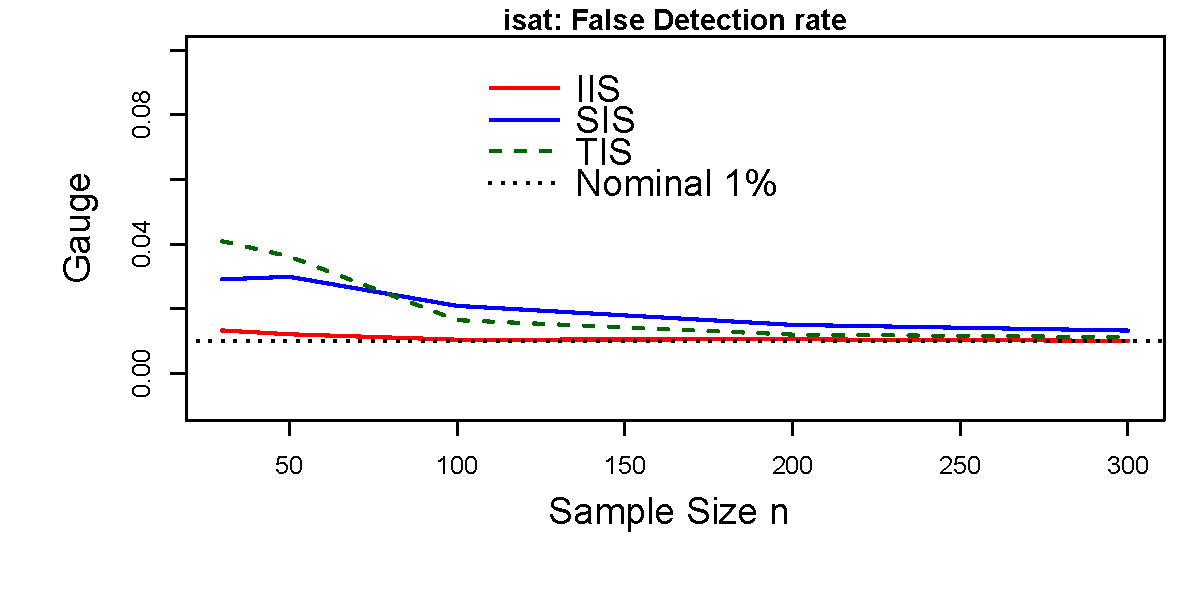
\includegraphics[width=0.7\textwidth, trim = 0 25 0 5, clip]{fig_isat_performance_v2.pdf}
  \caption{Gauge (false-detection rate) in IIS, SIS, TIS in
    \code{isat} under the null of no structural breaks or outliers for
    varying sample sizes $n$ at nominal selection significance of
    $\alpha=1\%$, using a static DGP of $y_t=u_t$ where
    $u_t \sim N(0, \sigma^2)$ with 1000 replications. The gauge
    approaches the nominal significance level of selection as
    $n \rightarrow \infty$. \label{fig_isat} }
\end{figure}
\subsection{Example: Structural breaks in the growth rate of UK SO$_2$ emissions}

Annual emissions of the pollutant sulphur dioxide (SO$_2$) in the UK
have declined in the latter half of the 20th century due to policy
interventions and changes in energy production. Here we assess whether
there have been significant shifts in the growth rate
($\Delta \log(SO_2)_t$) of sulphur dioxide emissions between 1946 and
2005, using SIS and the emission time series compiled by
\cite{smith2011anthropogenic}. Setting \code{t.pval} to 0.01 yields an
approximate gauge of $0.01k$ under the null hypothesis of no shifts
for $k$ spuriously included variables. Inclusion of a full set of
indicators implies that $k=n$ for IIS, and $k=n-1$ for SIS, and thus
$0.01(n-1) = 0.01 \times 59$. This suggests less than one indicator
being retained spuriously on average in a well-specified model under
the null of no shifts or outliers. Estimating an \code{isat} model
using SIS (\code{sis = TRUE} is default):
%
\begin{CodeChunk}
\begin{CodeInput}
R> options(plot = TRUE)
R> so2 <- data("so2data", package = "gets")  
R> yso2 <- zoo(so2data[, "DLuk_tot_so2"], order.by = so2data[, "year"])
R> (sis <- isat(yso2, t.pval = 0.01))
\end{CodeInput}
\begin{CodeOutput}
SIS block 1 of 2:
30 paths to search
Searching: 1 2 3 4 ...

SIS block 2 of 2:

26 paths to search
Searching: 1 2 3 4 ...

GETS of union of retained SIS variables... 
2 paths to search
Searching: 1 2 

...

SPECIFIC mean equation:

               coef   std.error    t-stat      p-value
mconst   0.01465385 0.007931984  1.847438 7.026836e-02
sis1972 -0.04332051 0.011866458 -3.650669 5.990412e-04
sis1993 -0.11693333 0.020126141 -5.810023 3.625832e-07
sis1998  0.12860000 0.044305650  2.902564 5.382516e-03
sis1999 -0.28400000 0.057198348 -4.965178 7.505854e-06
sis2000  0.24550000 0.045219264  5.429102 1.441154e-06
sis2004 -0.11550000 0.035026692 -3.297485 1.746083e-03

Diagnostics:

                   Chi-sq df p-value
Ljung-Box AR(1)   0.61553  1 0.43271
Ljung-Box ARCH(1) 1.44153  1 0.22989
Jarque-Bera       0.57302  2 0.75088
                          
SE of regression   0.04045
R-squared          0.73021
Log-lik.(n=60)   110.83192
\end{CodeOutput}
\end{CodeChunk}
%
The above output shows multiple detected step-shifts (labeled
\code{sis1972}--\code{sis2004}) in the time series. If plotting is
active (\code{plot = TRUE}), \code{isat}\ also displays the output as
in Figure~\ref{fig_sisso2} plotting the observed and fitted values,
together with the coefficient path (the time-varying intercept through
the regimes detected using SIS) as well as the standardized
residuals. There is a downward step-shift detected in the growth rate
in 1972, outlying observations are detected through two subsequent
step-indicators with opposite-signs (e.g., in 1998/1999), as well as a
downward step-shift at the end of the sample in 2004. This example
demonstrates the flexibility of the SIS approach -- step-shifts are
easily identified even at the end of the sample while outliers can be
detected simultaneously. The model can easily be extended to include
autoregressive terms using the \code{ar} argument, for example we
could estimate an AR(1) model with step-indicator saturation writing
\code{isat(yso2, ar = 1, t.pval = 0.01)}. Detection of outliers and 
structural breaks can be directly parallelized to increase 
computational speed when there are a large number of blocks searched 
over by setting the argument \code{parallel.options} equal to the 
number of cores available for processing. For example, 
\code{isat(yso2, t.pval = 0.01, parallel.options = 2)} estimates the 
above model in parallel using two cores.  

Additional covariates can be included in an IS regression model by
including them in the \code{mxreg} argument. If fixed regressors
entering through \code{mxreg} induce perfect collinear with break
functions in IS, then indicators are removed automatically before
selection. For example, consider forcing a hypothesized step-shift in
1972 to be retained while simultaneously searching for additional
shifts throughout the sample:
%
\begin{CodeChunk}
\begin{CodeInput}
R> x1972 <- zoo(sim(so2data[, "year"])[, 26], order.by = so2data[, "year"])
R> isat(yso2, t.pval = 0.01, mxreg = x1972)
\end{CodeInput}
\end{CodeChunk}
%
The resulting estimation does not select over the fixed step-shift in 1972, though for this particular example the estimated terminal model with a forced step shift matches the SIS results of a general search.
%
\begin{figure}[t!]
  \centering
  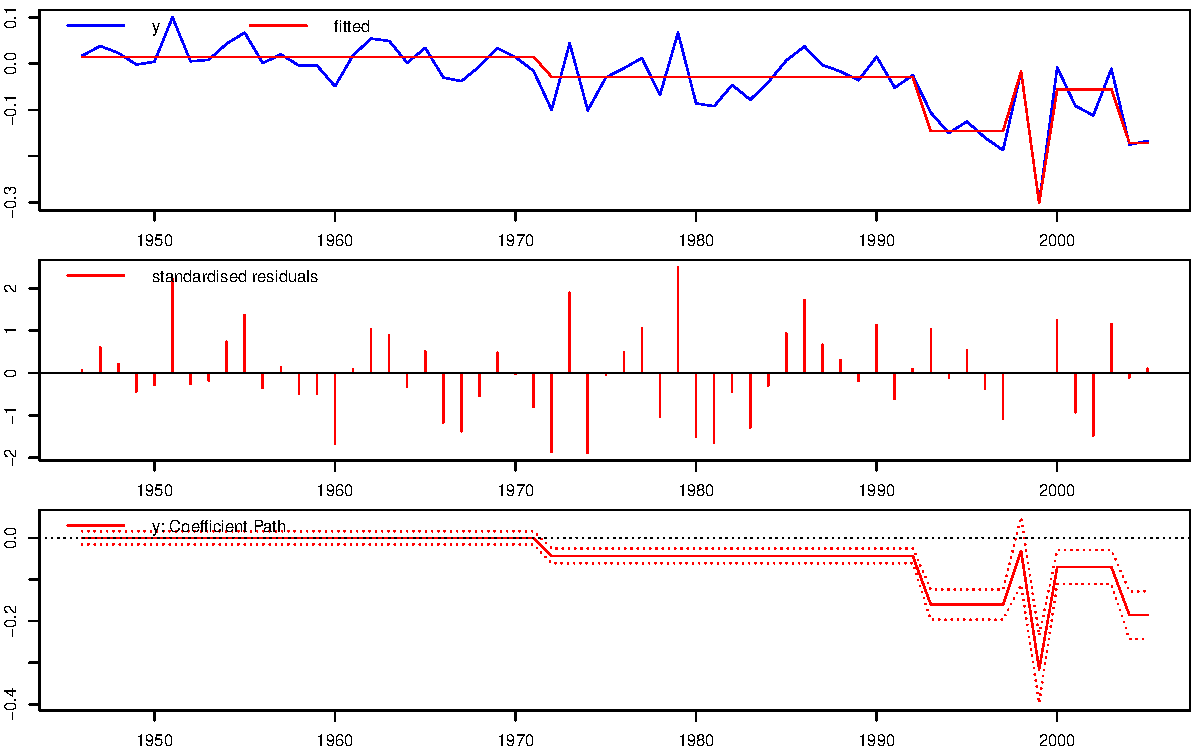
\includegraphics[scale=0.4]{fig_sis_so2_2.pdf}
  \caption{Annual UK SO$_2$ emission growth rate: step-indicator
    saturation model results. The top panel shows observed (blue) and fit
    time series (red). The middle panel shows the standardized residuals, the bottom panel
    shows the coefficient path relative to the intercept and its
    approximate 95\% confidence interval. \label{fig_sisso2} }
\end{figure}

\subsection{Testing and bias correcting post-model selection in indicator saturation}

The coefficient path describes how the value of a coefficient on a
particular variable evolves over time. The coefficient path of the
intercept of the `\code{isat}' object can be extracted using the
\code{isatvar} function. The function returns the coefficient path
both as the time-varying intercept (\code{const.path}) and as
deviation relative to the full-sample intercept (\code{coef.path}),
together with the approximate variance of the coefficient path
computed using the approach in \cite{pretis2015istest}. When the model
is specified to include autoregressive terms, then \code{isatvar}
(setting \code{lr = TRUE}) also returns the static long-run solution
of the dynamic model with its approximate variance.
%
\begin{CodeChunk}
\begin{CodeInput}
R> sisvar <- isatvar(sis)
R> sisvar
\end{CodeInput}
\begin{CodeOutput}
       coef.path  const.path    const.var    const.se
1946  0.00000000  0.01465385 6.291637e-05 0.007931984
1947  0.00000000  0.01465385 6.291637e-05 0.007931984
...
\end{CodeOutput}
\end{CodeChunk}
%
Indicator saturation may result in an under-estimation of the error
variance as observations are ``dummied out'' resulting in a truncation
of the distribution of the error terms. The magnitude of this effect
depends on the level of significance of selection and is generally
small for low values of $\alpha$. This effect manifests itself in an
under-estimation of the error variance, and an under-estimation of the
variance of regressors not selected over. Both can be corrected when
using IIS through consistency and efficiency correction factors
derived in \cite{johansen2016asymptotic}. These correction factors are
implemented in \pkg{gets} as functions \code{isvarcor} which corrects
the estimated error variance, and \code{isvareffcor} for an additional
correction on the estimated variance of fixed regressors. The
correction factors can be applied manually to estimation results, or
specified as arguments (\code{conscorr = TRUE} and
\code{effcorr = TRUE}) within the \code{isatvar} function. This is
demonstrated below running IIS on an autoregressive model with one lag
(\code{ar = 1}) on the growth rate of SO$_2$ emissions. The estimated
variance of the coefficient path is higher once consistency and
efficiency corrections are applied:
%
\begin{CodeChunk}
\begin{CodeInput}
R> iis <- isat(yso2, ar = 1, sis = FALSE, iis = TRUE, t.pval = 0.05)
R> isatvar(iis, conscorr = TRUE, effcorr = TRUE)
\end{CodeInput}
\begin{CodeOutput}
       coef.path   const.path    const.var    const.se
1947  0.00000000 -0.006210179 7.225479e-05 0.008500282
1948  0.00000000 -0.006210179 7.225479e-05 0.008500282
...
\end{CodeOutput}
\begin{CodeInput}
R> isatvar(iis,  conscorr = FALSE, effcorr = FALSE)
\end{CodeInput}
\begin{CodeOutput}
       coef.path   const.path    const.var    const.se
1947  0.00000000 -0.006210179 4.483453e-05 0.006695859
1948  0.00000000 -0.006210179 4.483453e-05 0.006695859
...
\end{CodeOutput}
\end{CodeChunk}
%
The terminal models of \code{isat} are the result of model selection, and may therefore lead to a selection bias in the coefficient estimates of selected variables. Post-selection bias-correction for orthogonal variables can be conducted using the method proposed in \cite{HendryKrolzig2005}. This is implemented as the function \code{biascorr}. Following \cite{pretis2015istest}, bias-correction of the coefficients in a SIS model can be directly applied to the coefficient path without prior orthogonalization. Bias-correcting the coefficient path of the above model of the growth rate of SO$_2$ yields the one- and two-step bias-corrected coefficients:
%
\begin{CodeChunk}
\begin{CodeInput}
R> bcorr <- biascorr(b = sisvar[, "const.path"], b.se = sisvar[, "const.se"],
+    p.alpha = 0.01, T = length(sisvar[, "const.path"]))
\end{CodeInput}
\begin{CodeOutput}
            beta  beta.1step  beta.2step
...
1997 -0.14560000 -0.14560000 -0.14560000
1998 -0.01700000 -0.01700000 -0.01700000
1999 -0.30100000 -0.30099983 -0.30099983
2000 -0.05550000 -0.04043232 -0.03000334
2001 -0.05550000 -0.04043232 -0.03000334
...	
\end{CodeOutput}
\end{CodeChunk}
%
Bias-correction reduces the magnitude of the estimated coefficients slightly to account for potential selection bias.

The function \code{isattest} makes it possible to conduct hypothesis
tests on the coefficient path of the intercept of an `\code{isat}'
object. This test is described in \cite{pretis2015istest} and builds
on \cite{ericsson2013biased} and \cite{pretis2015testing} who use
indicator saturation as a test for time-varying forecast accuracy. The
main arguments of the \code{isattest} function are:
%
\begin{itemize}
\item \code{hnull}: numeric. The null-hypothesis value to be tested against.

\item \code{lr}: logical. If \code{TRUE} and the `\code{isat}' object to be tested contains autoregressive terms, then the test is conducted on the long-run equilibrium coefficient path.

\item \code{ci.pval}: numeric, between 0 and 1. The level of significance for the confidence interval and hypothesis test.
	
\item \code{conscorr}: logical. If \code{TRUE} then the estimated error variance in IIS is consistency-corrected using the results in \cite{johansen2016asymptotic}.

\item \code{effcorr}: logical. If \code{TRUE} then the estimated variance of fixed regressors in IIS is efficiency corrected using the results in \cite{johansen2016asymptotic}.
	
\item \code{biascorr}: logical. If \code{TRUE} then the coefficient path is bias-corrected prior to testing. This is only valid for a non-dynamic (no auto-regressive terms) test without additional covariates.
\end{itemize}
%
Here we test the time-varying mean (as determined using SIS) of the annual growth rate of UK SO$_2$ emissions against the null hypothesis of zero-growth using \code{isattest}:
%
\begin{CodeChunk}
\begin{CodeInput}  
R> isattest(sis, hnull = 0, lr = FALSE, ci.pval = 0.99, plot.turn = TRUE,
+    biascorr = TRUE)
\end{CodeInput}
\begin{CodeOutput}
           ci.low      ci.high bias.high   bias.low
1946 -0.006539007  0.035846700         0  0.0000000
1947 -0.006539007  0.035846700         0  0.0000000
1948 -0.006539007  0.035846700         0  0.0000000
...
\end{CodeOutput}
\end{CodeChunk}
%
The results are shown in the automatically-generated plot given in Figure~\ref{fig_sistest} (the \code{plot.turn = TRUE} argument automatically adds the break dates into the plot in the lower panel). When testing at 1\% and using bias-correction this suggests that the detected shift in 1972 does not significantly move the growth-rate away from zero. Similarly, the upward shift in 2000 moves the growth rate back to zero. This change, however, is off-set by the shift at the end of the sample which shows the growth rate turning significantly negative in 2004.

\begin{figure}[t!]
  \centering
  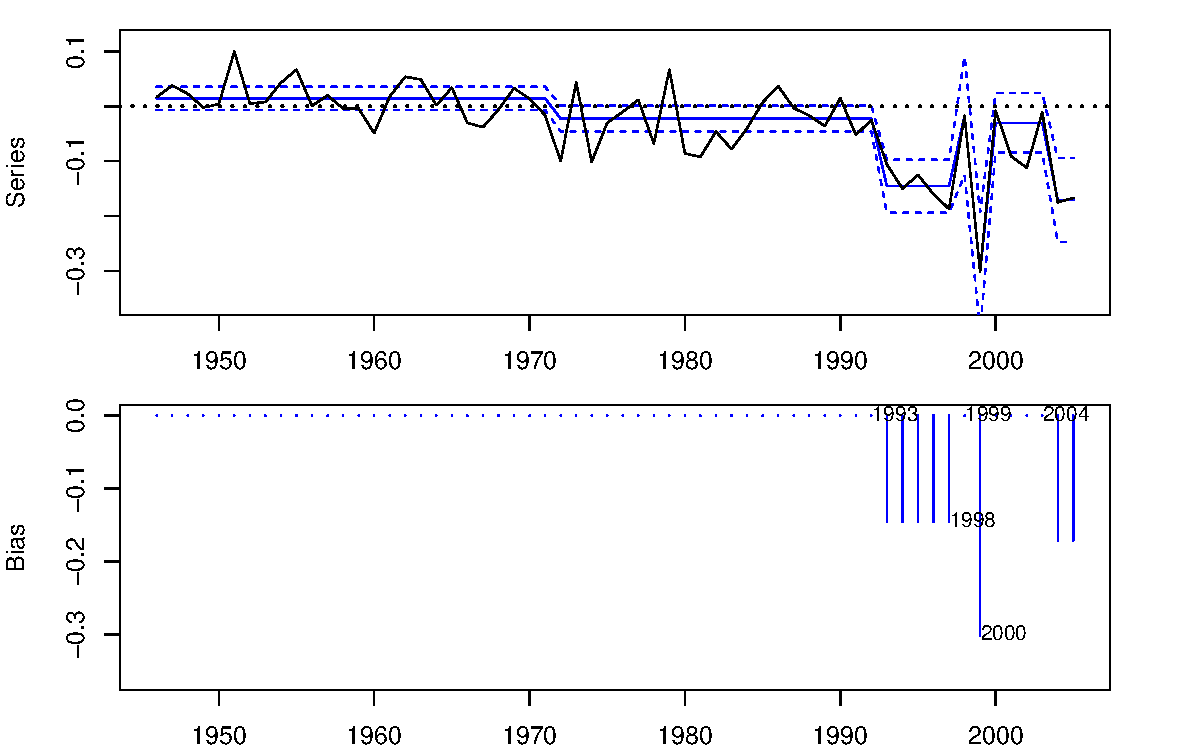
\includegraphics[scale=0.4]{fig_sis_test.pdf}
  \caption{Hypothesis test on the annual UK SO$_2$ emission growth
    rate following step-indicator saturation. The top panel shows observed
    (black) and bias-corrected fit (blue). The bottom panel shows the
    periods where the null-hypothesis is rejected, together with the
    dates of the significant breaks. \label{fig_sistest} }
\end{figure}

\subsection[Comparison of isat with other methods]{Comparison of \code{isat} with other methods}
\label{sec:isat_comp}

Indicator saturation formulates the detection of breaks and outliers as a problem of model (or variable) selection. Here we first provide an overview of software implementing indicator saturation, followed by a discussion of \code{isat} in \pkg{gets} relative to other existing break detection packages.

The only other currently existing software implementing indicator
saturation is \pkg{Autometrics}. IIS and SIS are available in both
\pkg{Autometrics} and \pkg{gets}, however, a crucial difference within
SIS is the construction and subsequent interpretation of
step-indicators. In \pkg{gets} steps are constructed as forward-steps:
${\bf S} = \left( 1_{\{t \geq j\}}, j=1,\ldots,n\right)$, where
$1_{\{t \geq j \}}$ denotes the indicator function such that
$1_{ \{t \geq j\}}=1$ for observations from $j$ onwards, and zero
otherwise. Thus the signs of the coefficients in the retained
regression model in \pkg{gets} correspond to the direction of the
step: positive (negative) coefficients imply an upward (downward)
step, and the coefficient path begins with the regression intercept
where for each subsequent regime the coefficient on the step indicator
is added to the full sample intercept. \pkg{Autometrics} relies on
backward-steps: ${\bf S} = \left( 1_{\{t \leq j\}}, j=1,\ldots,n\right)$
and thus step-coefficients have to be interpreted as opposite-signed
relative to the reported regression coefficients. \pkg{Autometrics}
currently has no implementation of the computation of the coefficient
path and its approximate variance, thus testing on the different
regimes is non-trivial. This is directly implemented in \pkg{gets} by
automatically plotting the coefficient path (if \code{plot = TRUE}),
which can be extracted using \code{isatvar}. The variance estimates in
\pkg{Autometrics} are currently not consistency or efficiency
corrected when using IS. This is implemented in \pkg{gets} and --
together with the extraction of the coefficient path and its variance
-- enables testing on the coefficient path using the \code{isattest}
function, together with automatic bias-correction if
specified. Further, automatic trend-indicator saturation (TIS) is
currently only available in \pkg{gets}. Both \pkg{Autometrics} and
\pkg{gets} enable the selection over designed break functions --
through the argument \code{uis} in \pkg{gets} and the general more
variables than observations model selection algorithm in
\pkg{Autometrics}.

In the broader field of detection of breaks or changepoints, the main difference to existing methods (e.g., \citealt{bai1998estimating}, \citealt{bai2003computation}, \citealt{perron2006dealing} implemented in \pkg{strucchange} by \citealt{kleiber2002strucchange}) or detection of changepoints in general (as in the package \pkg{changepoint} -- see \citealt{killick2014changepoint}) is the model-selection approach to break detection in indicator saturation (for discussion of methodological differences see \citealt{castle2015detecting}, as well as \citealt{HendryJohansenSantos2007}, and \citealt{johansen2016asymptotic}). This makes it possible to detect outliers (single period shifts) jointly with structural breaks (multiple period shifts), further it is also possible to detect breaks using designed functions \citep{pretis_volc16} which is not possible in conventional structural break methods or changepoint analysis. 

Where the indicator saturation methodology overlaps in applications
with existing methods is the detection of shifts in the intercept of
time series regression models, for example using \code{breakpoints} in
\pkg{strucchange}. Relative to \pkg{strucchange} and the Bai and
Perron least-squares approach in changes in the mean, \code{isat} in
\pkg{gets} does not impose a minimum break length and can therefore
conduct outlier detection jointly with shifts in the intercept,
further there is no implicit upper limit on the number of breaks, and
it is thus possible to identify outliers or shifts in the mean at the
start or end of samples as no trimming is required. Changes in
regression coefficients on random variables can be detected in
\code{isat} using designed break functions through the \code{uis}
argument by interacting a full set of step-indicators with the random
variable. This, however, is computationally expensive as each
additional variable whose coefficient is allowed to break over time
adds a set of $n$ variables to be selected over the GUM. The function
\code{breakpoints} in \pkg{strucchange} estimates a pure structural
change model where all coefficients change, \code{isat} in \pkg{gets}
is a partial model where the coefficients on variables included
through \code{mxreg} are not allowed to break, and only breaks in the
mean (or specified coefficients through inclusion in \code{uis}) are
permitted -- making it possible to pre-specify constancy. A partial
structural change model using the Bai and Perron least-squares
approach can be estimated using available \proglang{MATLAB}
code.\footnote{Available online at
  \url{http://people.bu.edu/perron/code.html}.}

Relative to \pkg{changepoint}, \code{isat} in \pkg{gets} is focused on
regression modeling and structural breaks in the intercept of
regression models jointly with outlier detection. As the authors of
\pkg{changepoint} themselves note, \pkg{changepoint} does not focus on
changes in regression models. The function \code{isat} directly
enables the inclusion of covariates through \code{mxreg} or \code{ar}
within \code{isat}, only if no additional covariates are specified
then \code{isat} searches for changes in the mean of a time series as
in the models used in the \pkg{changepoint} package while, however,
simultaneously detecting outliers.
	
\section[Exporting results to EViews, STATA, and LaTeX]{Exporting results to \proglang{EViews}, \proglang{STATA} and \LaTeX{}}
\label{sec:eviews:and:stata:export}
	
The two most popular commercial econometric software packages are
\proglang{EViews} \citep{EViews2016v9.5} and \proglang{STATA}
\citep{STATA2017}, but none of these provide GETS modeling
capabilities. To facilitate the usage of GETS modeling for
\proglang{EViews} and \proglang{STATA} users, we provide two functions
for this purpose, \code{eviews} and \code{stata}. Both functions work
in a similar way, and both can be applied on either `\code{arx}',
`\code{gets}' or `\code{isat}' objects. For example, typing
\code{eviews(getsm05)} yields the following print output:
%
\begin{CodeChunk}
\begin{CodeOutput}
EViews code to estimate the model:

  equation getsm05.ls(cov = white) yy mxreg4 

R code (example) to export the data of the model:

  eviews(getsm05, file = 'C:/Users/myname/Documents/getsdata.csv')
\end{CodeOutput}
\end{CodeChunk}
%
In other words, the code to estimate the final model in
\proglang{EViews}, and -- if needed -- a code-suggestion for how to
export the data of the model. The need to export the data of the final
model is likely to be most relevant subsequent to the use of
\code{isat}. The \code{stata} function works similarly. Note that both
the \code{eviews} and \code{stata} functions are only applicable to
conditional mean specifications, since neither \proglang{EViews} nor
\proglang{STATA} offer the estimation of dynamic log-variance models.

The objects returned by \code{arx}, \code{getsm}, \code{getsv} and
\code{isat} are lists. The entries in these lists that contain the
main estimation output are objects of class `\code{data.frame}'. That
means the \proglang{R} package \pkg{xtable} of \cite{Dahl2016} can be
used to generate \LaTeX{} code of the data frames.

\section{Conclusions}
\label{sec:conclusions}

The \proglang{R} package \pkg{gets} provides a toolkit for
general-to-specific modeling through automatic variable selection in
regression specifications of the mean and the variance, as well as
indicator saturation methods to detect outliers and structural
breaks. Starting with a general candidate set of variables unknown to
be relevant or irrelevant, selection using \code{getsm} or
\code{getsv} can yield parsimonious terminal models that satisfy a set
of chosen diagnostic criteria, where parameter changes and outlying
observations are detected using \code{isat}.
	
%\bibliography{ref}
\begin{thebibliography}{56}
	\newcommand{\enquote}[1]{``#1''}
	\providecommand{\natexlab}[1]{#1}
	\providecommand{\url}[1]{\texttt{#1}}
	\providecommand{\urlprefix}{URL }
	\expandafter\ifx\csname urlstyle\endcsname\relax
	\providecommand{\doi}[1]{doi:\discretionary{}{}{}#1}\else
	\providecommand{\doi}{doi:\discretionary{}{}{}\begingroup
		\urlstyle{rm}\Url}\fi
	\providecommand{\eprint}[2][]{\url{#2}}
	
	\bibitem[{Akaike(1974)}]{Akaike1974}
	Akaike H (1974).
	\newblock \enquote{A New Look at the Statistical Model Identification.}
	\newblock \emph{IEEE Transactions on Automatic Control}, \textbf{19}(6),
	716--723.
	\newblock \doi{10.1109/tac.1974.1100705}.
	
	\bibitem[{Bai and Perron(1998)}]{bai1998estimating}
	Bai J, Perron P (1998).
	\newblock \enquote{Estimating and Testing Linear Models with Multiple
		Structural Changes.}
	\newblock \emph{Econometrica}, \textbf{66}(1), 47--78.
	\newblock \doi{10.2307/2998540}.
	
	\bibitem[{Bai and Perron(2003)}]{bai2003computation}
	Bai J, Perron P (2003).
	\newblock \enquote{Computation and Analysis of Multiple Structural Change
		Models.}
	\newblock \emph{Journal of Applied Econometrics}, \textbf{18}(1), 1--22.
	\newblock \doi{10.1002/jae.659}.
	
	\bibitem[{Campos \emph{et~al.}(2005)Campos, Hendry, and
		Ericsson}]{CamposEricssonHendry2005}
	Campos J, Hendry DF, Ericsson NR (eds.) (2005).
	\newblock \emph{General-to-Specific Modeling. Volumes 1 and 2}.
	\newblock Edward Elgar Publishing, Cheltenham.
	
	\bibitem[{Castle \emph{et~al.}(2011)Castle, Doornik, and
		Hendry}]{castle2011evaluating}
	Castle JL, Doornik JA, Hendry DF (2011).
	\newblock \enquote{Evaluating Automatic Model Selection.}
	\newblock \emph{Journal of Time Series Econometrics}, \textbf{3}(1), 1--31.
	\newblock \doi{10.2202/1941-1928.1097}.
	
	\bibitem[{Castle \emph{et~al.}(2015)Castle, Doornik, Hendry, and
		Pretis}]{castle2015detecting}
	Castle JL, Doornik JA, Hendry DF, Pretis F (2015).
	\newblock \enquote{Detecting Location Shifts During Model Selection by
		Step-Indicator Saturation.}
	\newblock \emph{Econometrics}, \textbf{3}(2), 240--264.
	\newblock \doi{10.3390/econometrics3020240}.
	
	\bibitem[{Dahl(2016)}]{Dahl2016}
	Dahl DB (2016).
	\newblock \emph{\pkg{xtable}: Export Tables to \LaTeX{} or HTML}.
	\newblock \proglang{R} package version 1.8-2,
	\urlprefix\url{https://CRAN.R-project.org/package=xtable}.
	
	\bibitem[{Doornik(2006)}]{Doornik2006}
	Doornik J (2006).
	\newblock \emph{\proglang{Ox}: An Object Oriented Matrix Programming Language}.
	\newblock 5th edition. Timberlake Consultants Ltd., London.
	
	\bibitem[{Doornik(2009)}]{Doornik2009}
	Doornik J (2009).
	\newblock \enquote{\pkg{Autometrics}.}
	\newblock In JL~Castle, N~Shephard (eds.), \emph{The Methodology and Practice
		of Econometrics: A Festschrift in Honour of David F. {H}endry}, pp. 88--121.
	Oxford University Press, Oxford.
	
	\bibitem[{Doornik and Hendry(2007{\natexlab{a}})}]{DoornikHendry2007}
	Doornik JA, Hendry DF (2007{\natexlab{a}}).
	\newblock \emph{Empirical Econometric Modelling -- \pkg{PcGive} 12: Volume I}.
	\newblock Timberlake Consultants Ltd., London.
	
	\bibitem[{Doornik and Hendry(2007{\natexlab{b}})}]{DoornikHendry2007a}
	Doornik JA, Hendry DF (2007{\natexlab{b}}).
	\newblock \emph{Empirical Econometric Modelling -- \pkg{PcGive} 12: Volume II}.
	\newblock Timberlake Consultants Ltd., London.
	
	\bibitem[{Duan(1983)}]{Duan1983}
	Duan N (1983).
	\newblock \enquote{Smearing Estimate: A Nonparametric Retransformation Method.}
	\newblock \emph{Journal of the Americal Statistical Association},
	\textbf{78}(383), 605--610.
	\newblock \doi{10.2307/2288126}.
	
	\bibitem[{Efron \emph{et~al.}(2004)Efron, Hastie, Johnstone, and
		Tibshirani}]{efron2004least}
	Efron B, Hastie T, Johnstone I, Tibshirani R (2004).
	\newblock \enquote{Least Angle Regression.}
	\newblock \emph{The Annals of Statistics}, \textbf{32}(2), 407--499.
	\newblock \doi{10.1214/009053604000000067}.
	
	\bibitem[{Engle(1982)}]{Engle82}
	Engle R (1982).
	\newblock \enquote{Autoregressive Conditional Heteroscedasticity with Estimates
		of the Variance of United Kingdom Inflations.}
	\newblock \emph{Econometrica}, \textbf{50}(4), 987--1008.
	\newblock \doi{10.2307/1912773}.
	
	\bibitem[{Ericsson(2017)}]{ericsson2013biased}
	Ericsson NR (2017).
	\newblock \enquote{How Biased Are US Government Forecasts of the Federal Debt?}
	\newblock \emph{International Journal of Forecasting}, \textbf{33}(2),
	543--559.
	\newblock \doi{10.1016/j.ijforecast.2016.09.001}.
	
	\bibitem[{Francq and Sucarrat(2018)}]{FrancqSucarrat2013}
	Francq C, Sucarrat G (2018).
	\newblock \enquote{An Exponential Chi-Squared QMLE for Log-GARCH Models Via the
		ARMA Representation.}
	\newblock \emph{Journal of Financial Econometrics}, \textbf{16}(1), 129--154.
	\newblock \doi{10.1093/jjfinec/nbx032}.
	
	\bibitem[{Friedman \emph{et~al.}(2010)Friedman, Hastie, and
		Tibshirani}]{friedman2010regularization}
	Friedman J, Hastie T, Tibshirani R (2010).
	\newblock \enquote{Regularization Paths for Generalized Linear Models via
		Coordinate Descent.}
	\newblock \emph{Journal of Statistical Software}, \textbf{33}(1), 1--22.
	\newblock \doi{10.18637/jss.v033.i01}.
	
	\bibitem[{Glosten \emph{et~al.}(1993)Glosten, Jagannathan, and
		Runkle}]{GlostenJagannathanRunkle1993}
	Glosten LR, Jagannathan R, Runkle DE (1993).
	\newblock \enquote{On the Relation between the Expected Value and the
		Volatility of the Nominal Excess Return on Stocks.}
	\newblock \emph{Journal of Finance}, \textbf{48}(5), 1779--1801.
	\newblock \doi{10.2307/2329067}.
	
	\bibitem[{Hannan and Quinn(1979)}]{HannanQuinn1979}
	Hannan EJ, Quinn BG (1979).
	\newblock \enquote{The Determination of the Order of an Autoregression.}
	\newblock \emph{Journal of the Royal Statistical Society B}, \textbf{41}(2),
	190--195.
	
	\bibitem[{Hastie and Efron(2013)}]{HastieEfron2013}
	Hastie T, Efron B (2013).
	\newblock \emph{\pkg{lars}: Least Angle Regression, Lasso and Forward
		Stagewise}.
	\newblock \proglang{R} package version 1.2,
	\urlprefix\url{https://CRAN.R-project.org/package=lars}.
	
	\bibitem[{Hendry(2003)}]{Hendry03}
	Hendry DF (2003).
	\newblock \enquote{J. Denis Sargan and the Origins of LSE Econometric
		Methodology.}
	\newblock \emph{Econometric Theory}, \textbf{19}(3), 457--480.
	\newblock \doi{10.1017/s0266466603193061}.
	
	\bibitem[{Hendry and Doornik(2014)}]{HendryDoornik2014}
	Hendry DF, Doornik J (2014).
	\newblock \emph{Empirical Model Discovery and Theory Evaluation}.
	\newblock The MIT Press, London.
	
	\bibitem[{Hendry and Johansen(2015)}]{hendry2015model}
	Hendry DF, Johansen S (2015).
	\newblock \enquote{Model Discovery and Trygve Haavelmo's Legacy.}
	\newblock \emph{Econometric Theory}, \textbf{31}(1), 93--114.
	\newblock \doi{10.1017/s0266466614000218}.
	
	\bibitem[{Hendry \emph{et~al.}(2007)Hendry, Johansen, and
		Santos}]{HendryJohansenSantos2007}
	Hendry DF, Johansen S, Santos C (2007).
	\newblock \enquote{Automatic Selection of Indicators in a Fully Saturated
		Regression.}
	\newblock \emph{Computational Statistics}, \textbf{23}(2), 317--335.
	\newblock \doi{10.1007/s00180-007-0054-z}.
	
	\bibitem[{Hendry and Krolzig(2001)}]{Hendryetal01}
	Hendry DF, Krolzig HM (2001).
	\newblock \emph{Automatic Econometric Model Selection Using \pkg{PcGets}}.
	\newblock Timberlake Consultants Press, London.
	
	\bibitem[{Hendry and Krolzig(2005)}]{HendryKrolzig2005}
	Hendry DF, Krolzig HM (2005).
	\newblock \enquote{The Properties of Automatic Gets Modelling.}
	\newblock \emph{The Economic Journal}, \textbf{115}(502), C32--C61.
	\newblock \doi{10.1111/j.0013-0133.2005.00979.x}.
	
	\bibitem[{Hoover and Perez(1999)}]{Hooveretal99}
	Hoover KD, Perez SJ (1999).
	\newblock \enquote{Data Mining Reconsidered: Encompassing and the
		General-to-Specific Approach to Specification Search.}
	\newblock \emph{The Econometrics Journal}, \textbf{2}(2), 167--191.
	\newblock \doi{10.1111/1368-423x.00025}.
	
	\bibitem[{{IHS Markit}(2017)}]{EViews2016v9.5}
	{IHS Markit} (2017).
	\newblock \emph{\proglang{EViews} Version 9.5}.
	\newblock IHS Markit, Irvine, CA.
	\newblock \urlprefix\url{http://www.eviews.com/}.
	
	\bibitem[{Jarque and Bera(1980)}]{JarqueBera1980}
	Jarque C, Bera A (1980).
	\newblock \enquote{Efficient Tests for Normality, Homoskedasticity, and Serial
		Independence.}
	\newblock \emph{Economics Letters}, \textbf{6}(3), 255--259.
	\newblock \doi{10.1016/0165-1765(80)90024-5}.
	
	\bibitem[{Johansen and Nielsen(2016)}]{johansen2016asymptotic}
	Johansen S, Nielsen B (2016).
	\newblock \enquote{Asymptotic Theory of Outlier Detection Algorithms for Linear
		Time Series Regression Models.}
	\newblock \emph{Scandinavian Journal of Statistics}, \textbf{43}(2), 321--348.
	\newblock \doi{10.1111/sjos.12174}.
	
	\bibitem[{Killick and Eckley(2014)}]{killick2014changepoint}
	Killick R, Eckley I (2014).
	\newblock \enquote{\pkg{changepoint}: An \proglang{R} Package for Changepoint
		Analysis.}
	\newblock \emph{Journal of Statistical Software}, \textbf{58}(3), 1--19.
	\newblock \doi{10.18637/jss.v058.i03}.
	
	\bibitem[{Kleiber \emph{et~al.}(2002)Kleiber, Hornik, Leisch, and
		Zeileis}]{kleiber2002strucchange}
	Kleiber C, Hornik K, Leisch F, Zeileis A (2002).
	\newblock \enquote{\pkg{strucchange}: An \proglang{R} Package for Testing for
		Structural Change in Linear Regression Models.}
	\newblock \emph{Journal of Statistical Software}, \textbf{7}(2), 1--38.
	\newblock \doi{10.18637/jss.v007.i02}.
	
	\bibitem[{Ljung and Box(1978)}]{Ljungetal79}
	Ljung GM, Box GEP (1978).
	\newblock \enquote{On a Measure of Lack of Fit in Time Series Models.}
	\newblock \emph{Biometrika}, \textbf{65}(2), 297--303.
	\newblock \doi{10.2307/2335207}.
	
	\bibitem[{Lovell(1983)}]{Lovell83}
	Lovell MC (1983).
	\newblock \enquote{Data Mining.}
	\newblock \emph{The Review of Economics and Statistics}, \textbf{65}(1), 1--12.
	\newblock \doi{10.2307/1924403}.
	
	\bibitem[{Mizon(1995)}]{Mizon95}
	Mizon G (1995).
	\newblock \enquote{Progressive Modeling of Macroeconomic Time Series: The LSE
		Methodology.}
	\newblock In KD~Hoover (ed.), \emph{Macroeconometrics. Developments, Tensions
		and Prospects}, pp. 107--169. Kluwer Academic Publishers, Dordrecht.
	
	\bibitem[{Newey and West(1987)}]{Neweyetal87}
	Newey W, West K (1987).
	\newblock \enquote{A Simple Positive Semi-Definite, Heteroskedasticity and
		Autocorrelation Consistent Covariance Matrix.}
	\newblock \emph{Econometrica}, \textbf{55}(3), 703--708.
	\newblock \doi{10.2307/1913610}.
	
	\bibitem[{Perron(2006)}]{perron2006dealing}
	Perron P (2006).
	\newblock \enquote{Dealing with Structural Breaks.}
	\newblock In H~Hassani, TC~Mills, K~Patterson (eds.), \emph{Palgrave Handbook
		of Econometrics: Volume 1}, pp. 278--352. Palgrave MacMillan, Hampshire, UK.
	
	\bibitem[{Pretis(2017)}]{pretis2015istest}
	Pretis F (2017).
	\newblock \enquote{Classifying Time-Varying Predictive Accuracy in Using
		Bias-Corrected Indicator Saturation.}
	\newblock University of Oxford Economics Discussion Paper.
	
	\bibitem[{Pretis and Jiao(2017)}]{pretis2017gauge}
	Pretis F, Jiao X (2017).
	\newblock \enquote{Testing the Presence of Outliers to Assess Misspecification
		in Regression Models.}
	\newblock University of Oxford Economics Discussion Paper.
	
	\bibitem[{Pretis \emph{et~al.}(2015)Pretis, Mann, and
		Kaufmann}]{pretis2015testing}
	Pretis F, Mann ML, Kaufmann RK (2015).
	\newblock \enquote{Testing Competing Models of the Temperature Hiatus:
		Assessing the Effects of Conditioning Variables and Temporal Uncertainties
		Through Sample-Wide Break Detection.}
	\newblock \emph{Climatic Change}, \textbf{131}(4), 705--718.
	\newblock \doi{10.1007/s10584-015-1391-5}.
	
	\bibitem[{Pretis \emph{et~al.}(2016)Pretis, Schneider, Smerdon, and
		Hendry}]{pretis_volc16}
	Pretis F, Schneider L, Smerdon JE, Hendry DF (2016).
	\newblock \enquote{Detecting Volcanic Eruptions in Temperature Reconstructions
		by Designed Break-Indicator Saturation.}
	\newblock \emph{Journal of Economic Surveys}, \textbf{30}(3), 403--429.
	\newblock \doi{10.1111/joes.12148}.
	
	\bibitem[{{\proglang{R} Core Team}(2018)}]{RCoreTeam2016}
	{\proglang{R} Core Team} (2018).
	\newblock \emph{\proglang{R}: A Language and Environment for Statistical
		Computing}.
	\newblock \proglang{R} Foundation for Statistical Computing, Vienna, Austria.
	\newblock \urlprefix\url{https://www.R-project.org/}.
	
	\bibitem[{Schneider \emph{et~al.}(2017)Schneider, Smerdon, Pretis, Hartl-Meier,
		and Esper}]{schneider2017}
	Schneider L, Smerdon J, Pretis F, Hartl-Meier C, Esper J (2017).
	\newblock \enquote{A New Archive of Large Volcanic Events Over the Past
		Millennium Derived from Reconstructed Summer Temperatures.}
	\newblock \emph{Environmental Research Letters}, \textbf{12}(9), 094005.
	\newblock \doi{10.1088/1748-9326/aa7a1b}.
	
	\bibitem[{Schwarz(1978)}]{Schwarz1978}
	Schwarz G (1978).
	\newblock \enquote{Estimating the Dimension of a Model.}
	\newblock \emph{The Annals of Statistics}, \textbf{6}(2), 461--464.
	\newblock \doi{10.1214/aos/1176344136}.
	
	\bibitem[{Smith \emph{et~al.}(2011)Smith, {van Aardenne}, Klimont, Andres,
		Volke, and {Delgado Arias}}]{smith2011anthropogenic}
	Smith SJ, {van Aardenne} J, Klimont Z, Andres RJ, Volke A, {Delgado Arias} S
	(2011).
	\newblock \enquote{Anthropogenic Sulfur Dioxide Emissions: 1850--2005.}
	\newblock \emph{Atmospheric Chemistry and Physics}, \textbf{11}(3), 1101--1116.
	\newblock \doi{10.5194/acp-11-1101-2011}.
	
	\bibitem[{{StataCorp}(2017)}]{STATA2017}
	{StataCorp} (2017).
	\newblock \emph{\proglang{STATA} Statistical Software: Release~15}.
	\newblock StataCorp LLC, College Station, TX.
	\newblock \urlprefix\url{http://www.stata.com/}.
	
	\bibitem[{Sucarrat(2010)}]{Sucarrat2010}
	Sucarrat G (2010).
	\newblock \enquote{Econometric Reduction Theory and Philosophy.}
	\newblock \emph{Journal of Economic Methodology}, \textbf{17}(1), 53--75.
	\newblock \doi{10.1080/13501780903528978}.
	
	\bibitem[{Sucarrat(2015{\natexlab{a}})}]{AutoSEARCH}
	Sucarrat G (2015{\natexlab{a}}).
	\newblock \emph{\pkg{AutoSEARCH}: General-to-Specific (GETS) Modelling}.
	\newblock \proglang{R} package version 1.5,
	\urlprefix\url{https://CRAN.R-project.org/package=AutoSEARCH}.
	
	\bibitem[{Sucarrat(2015{\natexlab{b}})}]{Sucarrat2015lgarchV06}
	Sucarrat G (2015{\natexlab{b}}).
	\newblock \emph{\pkg{lgarch}: Simulation and Estimation of Log-GARCH Models}.
	\newblock \proglang{R} package version 0.6-2,
	\urlprefix\url{https://CRAN.R-project.org/package=lgarch/}.
	
	\bibitem[{Sucarrat and Escribano(2012)}]{SucarratEscribano2012}
	Sucarrat G, Escribano {\'A} (2012).
	\newblock \enquote{Automated Model Selection in Finance: General-to-Specific
		Modelling of the Mean and Volatility Specifications.}
	\newblock \emph{Oxford Bulletin of Economics and Statistics}, \textbf{74}(5),
	716--735.
	\newblock \doi{10.1111/j.1468-0084.2011.00669.x}.
	
	\bibitem[{Sucarrat \emph{et~al.}(2016)Sucarrat, Gr{\o}nneberg, and
		Escribano}]{SucarratGronnebergEscribano2016}
	Sucarrat G, Gr{\o}nneberg S, Escribano {\'A} (2016).
	\newblock \enquote{Estimation and Inference in Univariate and Multivariate
		Log-GARCH-X Models When the Conditional Density Is Unknown.}
	\newblock \emph{Computational Statistics \& Data Analysis}, \textbf{100},
	582--594.
	\newblock \doi{10.1016/j.csda.2015.12.005}.
	
	\bibitem[{Sucarrat \emph{et~al.}(2018)Sucarrat, Pretis, and Reade}]{gets}
	Sucarrat G, Pretis F, Reade J (2018).
	\newblock \emph{\pkg{gets}: General-to-Specific (GETS) Modelling and Indicator
		Saturation Methods}.
	\newblock \proglang{R} package version 0.15,
	\urlprefix\url{https://CRAN.R-project.org/package=gets}.
	
	\bibitem[{{The~MathWorks Inc.}(2017)}]{MATLABR2017b}
	{The~MathWorks Inc} (2017).
	\newblock \emph{\proglang{MATLAB} -- The Language of Technical Computing,
		Version R2017b.}
	\newblock Natick, Massachusetts.
	\newblock \urlprefix\url{http://www.mathworks.com/products/matlab/}.
	
	\bibitem[{Tibshirani(1996)}]{tibshirani1996regression}
	Tibshirani R (1996).
	\newblock \enquote{Regression Shrinkage and Selection via the Lasso.}
	\newblock \emph{Journal of the Royal Statistical Society B}, \textbf{58}(1),
	267--288.
	
	\bibitem[{White(1980)}]{White80}
	White H (1980).
	\newblock \enquote{A Heteroskedasticity-Consistent Covariance Matrix and a
		Direct Test for Heteroskedasticity.}
	\newblock \emph{Econometrica}, \textbf{48}(4), 817--838.
	\newblock \doi{10.2307/1912934}.
	
	\bibitem[{Zeileis and Grothendieck(2005)}]{ZeileisGrothendieck2005}
	Zeileis A, Grothendieck G (2005).
	\newblock \enquote{\pkg{zoo}: \proglang{S}3 Infrastructure for Regular and
		Irregular Time Series.}
	\newblock \emph{Journal of Statistical Software}, \textbf{14}(6), 1--27.
	\newblock \doi{10.18637/jss.v014.i06}.
	
\end{thebibliography}

\newpage
\appendix
\section[Hoover and Perez (1999) simulations]{\cite{Hooveretal99} simulations} \label{appendix} 

Table~\ref{table:list 1 of experiments} contains the list of
experiments.  The design of the experiments HP1, HP2' and HP7' are
based on \citet[][see Table 3 on p.~174]{Hooveretal99}, and make use
of their data $x_{1t}^{\text{HP}},\ldots,x_{36t}^{\text{HP}}$. It
should be noted that there are two typos in their Table 3. The value
$\sqrt{(7/4)}$ should instead be $\sqrt{7}/4$ in the model of the
autoregressive error, and the value 6.73 should instead be 6.44 in
model 7', see also \citet{Doornik2009}. The number of relevant
variables in the GUM is $k_{\text{rel}}$, the number of irrelevant
variables in the GUM is $k_{\text{irr}}$ and the total number of
variables (the constant included) in the GUM is
$k = k_{\text{rel}} + k_{\text{irr}} + 1$. Nominal regressor
significance level used is 5\%, and 1000
replications. The term $m(\hat{k}_{\text{rel}}/k_{\text{rel}})$ is the average
proportion of relevant variables $\hat{k}_{\text{rel}}$ retained
relative to the actual number of relevant variables $k_{\text{rel}}$
in the DGP. The term $m(\hat{k}_{\text{irr}}/k_{\text{irr}})$ denotes the average
proportion of irrelevant variables $\hat{k}_{\text{irr}}$ retained
relative to the actual number of irrelevant variables $k_{\text{irr}}$
in the GUM. The estimate $\hat{k}_{\text{irr}}$ includes both
significant and insignificant retained irrelevant variables (this is
in line with \citet{HendryKrolzig2005}, and \citet{Doornik2009}, but
counter to HP which only includes significant irrelevant variables in
the estimate). $\hat{p}(\text{DGP})$ is the proportion of times the
DGP is found exactly. The properties of the HP algorithm are from
\citet[][Table 4 on p.~179]{Hooveretal99}. The properties of the
\pkg{PcGets} algorithm are from \citet[][Figure 1 on
p.~C39]{HendryKrolzig2005}, and the properties of the Autometrics
algorithm are from \citet[][Section 6]{Doornik2009}. For
\pkg{AutoSEARCH}, a constant is included in all the regressions but
ignored in the evaluation of successes and failures (this is in line
with \citet{Hooveretal99} but counter to \citet{HendryKrolzig2005},
and \citet{Doornik2009}), in the diagnostic checks both the AR and
ARCH test of the standardized residuals were undertaken at lag 2 using
a significance level of 2.5\% for each, and as tiebreaker the Schwarz
information criterion is used with a Gaussian log-likelihood made up
of the standardized residuals of the mean specification.

\begin{table}[t!]
  \centering
  \begin{tabular}{lccll}
    \hline
    Label & $k_{\text{rel}}$ & $k_{\text{irr}}$ & Simulation DGP & GUM \\
    \hline
    HP1 & 0 & 40 & \parbox[t]{.45\linewidth}{ $r_t=\epsilon_t, \\ \epsilon_t = 130z_t, \quad z_t\stackrel{\text{iid}}{\sim} N(0,1)$ } & \parbox[t]{.28\linewidth}{ $r_t =  \sum_{k=1}^{41}\psi_kx_{kt}^{\text{HP}} + \epsilon_t$,\\ where $x_{37t}^{\text{HP}} = r_{t-1}$,\\[2pt]
    $x_{38t}^{\text{HP}} = r_{t-2}$,
    $x_{39t}^{\text{HP}} = r_{t-3}$,\\[2pt]
    $x_{40t}^{\text{HP}} = r_{t-4}$ and
    $x_{41t}^{\text{HP}} = 1$ }\\
          & & & & \\
    HP2' & 1 & 39 & \parbox[t]{.45\linewidth}{ $r_t=0.75r_{t-1} + \epsilon_t, \\ \epsilon_t=85.99z_t, \quad z_t\stackrel{\text{iid}}{\sim} N(0,1)$ } & Same as in HP1. \\
          & & & & \\
    HP7' & 3 & 37 & \parbox[t]{.45\linewidth}{ $r_t = 0.75r_{t-1} + 1.33x_{11t}^{\text{HP}} - 0.9975x_{29t}^{\text{HP}} + \epsilon_t$, \\ $\epsilon_t=6.44z_t,\hspace{3mm}z_t\stackrel{\text{iid}}{\sim} N(0,1)$} & Same as in HP1.\\
    \hline
  \end{tabular}
  \caption{List of experiments.\label{table:list 1 of experiments} }
\end{table}
	
\section{Simulation tables}\label{sec:simulation-tables}

Tables~\ref{tab_lassuncorr}, \ref{tab_lassposcorr},
\ref{tab_lassnegcorr} and \ref{tab_isatgauge} present the simulation
results comparing \pkg{gets} to alternative variable selection
methods, and the properties of \code{isat} under the null of no
breaks.

\begin{table}[t!]
\centering
\begin{tabular}{rrrrrr|rrrrr}
\hline
    \multicolumn{2}{c}{$\rho=0$} & \multicolumn{4}{c}{Gauge,  $m(\widehat{k}_{\text{irr}}/k_{\text{irr}})$} & \multicolumn{5}{c}{Potency, $m(\widehat{k}_{\text{rel}}/k_{\text{rel}})$ } \\
\hline    
    \multicolumn{1}{l}{$k_{\text{rel}}$} & \multicolumn{1}{l}{$k_{\text{irr}}$} & \multicolumn{1}{l}{\code{getsm}} & \multicolumn{1}{l}{LassCV} & \multicolumn{1}{l}{LassFix} & \multicolumn{1}{l}{1-cut} & \multicolumn{1}{|l}{\code{getsm}} & \multicolumn{1}{l}{LassCV} & \multicolumn{1}{l}{LassFix} & \multicolumn{1}{l}{1-cut} & \multicolumn{1}{l}{DGP} \\ \hline 
     0 &   20 & 0.012 & 0.081 & 0.014 & 0.010 &  &  &  &  &  \\ 
     1 &   19 & 0.013 & 0.138 & 0.018 & 0.011 & 0.623 & 0.779 & 0.657 & 0.507 & 0.616 \\ 
     2 &   18 & 0.014 & 0.206 & 0.021 & 0.010 & 0.619 & 0.875 & 0.690 & 0.498 & 0.616 \\ 
     3 &   17 & 0.015 & 0.272 & 0.024 & 0.011 & 0.635 & 0.913 & 0.705 & 0.544 & 0.639 \\ 
     4 &   16 & 0.015 & 0.324 & 0.027 & 0.010 & 0.607 & 0.929 & 0.675 & 0.509 & 0.615 \\ 
     5 &   15 & 0.014 & 0.359 & 0.026 & 0.010 & 0.593 & 0.938 & 0.667 & 0.505 & 0.604 \\ 
     6 &   14 & 0.017 & 0.425 & 0.032 & 0.011 & 0.592 & 0.955 & 0.659 & 0.513 & 0.602 \\ 
     7 &   13 & 0.020 & 0.463 & 0.034 & 0.011 & 0.591 & 0.967 & 0.660 & 0.517 & 0.597 \\ 
     8 &   12 & 0.020 & 0.517 & 0.038 & 0.011 & 0.589 & 0.965 & 0.642 & 0.520 & 0.591 \\ 
     9 &   11 & 0.021 & 0.568 & 0.038 & 0.008 & 0.592 & 0.975 & 0.653 & 0.516 & 0.587 \\ 
    10 &   10 & 0.025 & 0.587 & 0.040 & 0.010 & 0.588 & 0.977 & 0.628 & 0.507 & 0.576 \\ 
\hline    
\end{tabular}
\caption{Variable selection properties of \code{getsm} algorithm in \pkg{gets} compared to alternative algorithms when regressors are uncorrelated in expectation. Variable selection in \code{getsm} is undertaken with a nominal significance level of 1\%. For a total number of $k=20$ variables, $m(\widehat{k}_{\text{rel}}/k_{\text{rel}})$ defines the average proportion of relevant variables $\widehat{k}_{\text{rel}}$ retained relative to the actual number of relevant variables $k_{\text{rel}}$. $m(\widehat{k}_{\text{irr}}/k_{\text{irr}})$, average proportion of irrelevant variables $\widehat{k}_{\text{irr}}$ retained relative to the actual number of irrelevant variables $k_{\text{irr}}$ in the GUM. LassCV denotes the the cross-validated LASSO using \pkg{glmnet}, LassFix denotes the LASSO where the penalty parameter is chosen to match the gauge of \code{getsm} under the null. Column 1-cut denotes 1-cut selection of the GUM where all variables with $p$~values $< 1$\% are retained in a single decision, DGP denotes the proportion of variables retained if the DGP is correctly estimated and $t$-tests are conducted at the 1\% level. Simulation undertaken on a sample of $n=100$ observations using 1000 replications. \label{tab_lassuncorr} }
\end{table}

\begin{table}[t!]
\centering
\begin{tabular}{rrrrrr|rrrrr}
    \hline 
    \multicolumn{2}{c}{$\rho=0.5$} & \multicolumn{4}{c}{Gauge,  $m(\widehat{k}_{\text{irr}}/k_{\text{irr}})$} & \multicolumn{5}{c}{Potency, $m(\widehat{k}_{\text{rel}}/k_{\text{rel}})$ } \\ \hline 
    \multicolumn{1}{l}{$k_{\text{rel}}$} & \multicolumn{1}{l}{$k_{\text{irr}}$} & \multicolumn{1}{l}{\code{getsm}} & \multicolumn{1}{l}{LassCV} & \multicolumn{1}{l}{LassFix} & \multicolumn{1}{l}{1-cut} & \multicolumn{1}{|l}{\code{getsm}} & \multicolumn{1}{l}{LassCV} & \multicolumn{1}{l}{LassFix} & \multicolumn{1}{l}{1-cut} & \multicolumn{1}{l}{DGP}  \\ \hline 
     0 &   20 & 0.018 & 0.074 & 0.009 & 0.011 &  &  &  &  &  \\ 
     1 &   19 & 0.025 & 0.154 & 0.043 & 0.009 & 0.502 & 0.752 & 0.616 & 0.257 & 0.654 \\ 
     2 &   18 & 0.026 & 0.232 & 0.095 & 0.010 & 0.505 & 0.874 & 0.782 & 0.258 & 0.498 \\ 
     3 &   17 & 0.029 & 0.273 & 0.139 & 0.009 & 0.508 & 0.911 & 0.847 & 0.248 & 0.418 \\ 
     4 &   16 & 0.031 & 0.307 & 0.169 & 0.010 & 0.525 & 0.921 & 0.870 & 0.262 & 0.388 \\ 
     5 &   15 & 0.032 & 0.338 & 0.202 & 0.010 & 0.522 & 0.932 & 0.887 & 0.247 & 0.353 \\ 
     6 &   14 & 0.038 & 0.378 & 0.229 & 0.011 & 0.525 & 0.938 & 0.899 & 0.255 & 0.344 \\ 
     7 &   13 & 0.036 & 0.394 & 0.249 & 0.009 & 0.536 & 0.946 & 0.912 & 0.263 & 0.336 \\ 
     8 &   12 & 0.043 & 0.421 & 0.281 & 0.010 & 0.523 & 0.947 & 0.915 & 0.251 & 0.328 \\ 
     9 &   11 & 0.046 & 0.440 & 0.305 & 0.011 & 0.527 & 0.954 & 0.928 & 0.250 & 0.315 \\ 
    10 &   10 & 0.048 & 0.447 & 0.304 & 0.011 & 0.526 & 0.958 & 0.933 & 0.254 & 0.308 \\ 
\hline 
\end{tabular}
\caption{Variable selection properties of \code{getsm} algorithm in \pkg{gets} compared to alternative algorithms when regressors are positively correlated ($\rho=0.5$) in expectation. Variable selection in \code{getsm} is undertaken with a nominal significance level of 1\%. For a total number of $k=20$ variables, $m(\widehat{k}_{\text{rel}}/k_{\text{rel}})$ defines the average proportion of relevant variables $\widehat{k}_{\text{rel}}$ retained relative to the actual number of relevant variables $k_{\text{rel}}$. $m(\widehat{k}_{\text{irr}}/k_{\text{irr}})$, average proportion of irrelevant variables $\widehat{k}_{\text{irr}}$ retained relative to the actual number of irrelevant variables $k_{\text{irr}}$ in the GUM. LassCV denotes the the cross-validated LASSO using \pkg{glmnet}, LassFix denotes the LASSO where the penalty parameter is chosen to match the gauge of \code{getsm} under the null. Column 1-cut denotes 1-cut selection of the GUM where all variables with $p$~values $<1$\% are retained in a single decision, DGP denotes the proportion of variables retained if the DGP is correctly estimated and $t$-tests are conducted at the 1\% level. Simulation undertaken on a sample of $n=100$ observations using 1000 replications. \label{tab_lassposcorr} }
\end{table}

\begin{table}[t!]
\centering
\begin{tabular}{rrrrrr|rrrrr}
\hline 
    \multicolumn{2}{c}{$\rho= \pm 0.5$} & \multicolumn{4}{c}{Gauge,  $m(\widehat{k}_{\text{irr}}/k_{\text{irr}})$} & \multicolumn{5}{c}{Potency, $m(\widehat{k}_{\text{rel}}/k_{\text{rel}})$ } \\ \hline 
    \multicolumn{1}{l}{$k_{\text{rel}}$} & \multicolumn{1}{l}{$k_{\text{irr}}$} & \multicolumn{1}{l}{\code{getsm}} & \multicolumn{1}{l}{LassCV} & \multicolumn{1}{l}{LassFix} & \multicolumn{1}{l}{1-cut} & \multicolumn{1}{|l}{\code{getsm}} & \multicolumn{1}{l}{LassCV} & \multicolumn{1}{l}{LassFix} & \multicolumn{1}{l}{1-cut} & \multicolumn{1}{l}{DGP} \\ \hline 
   0 &   20 & 0.018 & 0.080 & 0.010 & 0.010 &  &  &  &  &  \\ 
     1 &   19 & 0.023 & 0.156 & 0.041 & 0.011 & 0.505 & 0.756 & 0.602 & 0.255 & 0.635 \\ 
     2 &   18 & 0.022 & 0.165 & 0.009 & 0.009 & 0.376 & 0.558 & 0.172 & 0.241 & 0.457 \\ 
     3 &   17 & 0.025 & 0.218 & 0.035 & 0.008 & 0.393 & 0.695 & 0.360 & 0.254 & 0.409 \\ 
     4 &   16 & 0.023 & 0.259 & 0.008 & 0.010 & 0.375 & 0.685 & 0.168 & 0.253 & 0.385 \\ 
     5 &   15 & 0.026 & 0.309 & 0.026 & 0.009 & 0.375 & 0.751 & 0.296 & 0.262 & 0.369 \\ 
     6 &   14 & 0.024 & 0.353 & 0.008 & 0.010 & 0.369 & 0.765 & 0.181 & 0.255 & 0.354 \\ 
     7 &   13 & 0.027 & 0.387 & 0.026 & 0.009 & 0.356 & 0.807 & 0.259 & 0.249 & 0.336 \\ 
     8 &   12 & 0.029 & 0.418 & 0.012 & 0.011 & 0.339 & 0.806 & 0.164 & 0.249 & 0.316 \\ 
     9 &   11 & 0.032 & 0.464 & 0.023 & 0.010 & 0.355 & 0.846 & 0.244 & 0.255 & 0.322 \\ 
    10 &   10 & 0.031 & 0.484 & 0.012 & 0.010 & 0.347 & 0.849 & 0.174 & 0.246 & 0.306 \\ 
\hline 
\end{tabular}
\caption{Variable selection properties of \code{getsm} algorithm in
  \pkg{gets} compared to alternative algorithms when regressors are
  alternatingly positively and negatively correlated ($\rho= \pm 0.5$)
  in expectation. Variable selection in \code{getsm} is undertaken
  with a nominal significance level of 1\%. For a total number of
  $k=20$ variables, $m(\widehat{k}_{\text{rel}}/k_{\text{rel}})$
  defines the average proportion of relevant variables
  $\widehat{k}_{\text{rel}}$ retained relative to the actual number of
  relevant variables
  $k_{\text{rel}}$. $m(\widehat{k}_{\text{irr}}/k_{\text{irr}})$,
  average proportion of irrelevant variables
  $\widehat{k}_{\text{irr}}$ retained relative to the actual number of
  irrelevant variables $k_{\text{irr}}$ in the GUM. LassCV denotes the
  the cross-validated LASSO using \pkg{glmnet}, LassFix denotes the
  LASSO where the penalty parameter is chosen to match the gauge of
  \code{getsm} under the null. Column 1-cut denotes 1-cut selection of
  the GUM where all variables with $p$~values $\leq 1$\% are retained
  in a single decision, DGP denotes the proportion of variables
  retained if the DGP is correctly estimated and $t$-tests are
  conducted at the 1\% level. Simulation undertaken on a sample of
  $n=100$ observations using 1000
  replications. \label{tab_lassnegcorr} }
\end{table}
		
\begin{table}[t!]
  \centering
    \begin{tabular}{rrrr}
    		\hline 	
    \multicolumn{1}{l}{No.~breaks} & \multicolumn{3}{c}{Gauge,  $m(\widehat{k}_{\text{irr}}/k_{\text{irr}})$} \\ 		\hline
    \multicolumn{1}{l}{Sample $n$} & \multicolumn{1}{l}{IIS} & \multicolumn{1}{l}{SIS} & \multicolumn{1}{l}{TIS} \\ 		\hline
    30    & 0.013 & 0.028 & 0.042 \\
    50    & 0.012 & 0.029 & 0.037 \\
    100   & 0.011 & 0.019 & 0.016 \\
    200   & 0.011 & 0.015 & 0.011 \\
    300   & 0.010 & 0.013 & 0.011 \\ 		\hline
    \end{tabular}%
    \caption{Gauge (false-detection rate) in IIS, SIS, TIS in \code{isat} under the null of no structural breaks or outliers for varying sample sizes $n$ at nominal selection significance of $\alpha=1\%$ using a static DGP of $y_t=u_t$ where $u_t \sim N(0, \sigma^2)$ with 1000 replications. \label{tab_isatgauge} }
\end{table}	
		
\end{document}
